\chapter{習得事項}
\section{OSS・Linuxに対するソフトウェア検証手法・ツールの調査}
\label{tool}
本節では、OSS・Linuxシステムのソフトウェア検証に関する技法またはツールについて、SIL2LinuxMPプロジェクトで採用が検討されている%オープンソースライセンスの
ものを中心に調査結果を記載する。
前述のように、品質管理ライフサイクルにおいてはテスト実行のみにとどまらずテストケース生成、バグ抽出(\acrshort{fp}フィルタリング)、バグレポート生成、バグ管理、メトリクス測定・テストレポート生成など様々なタスクを実施する必要がある(図\ref{QA_Tasks})。
\begin{figure}[ht]
  \centering
  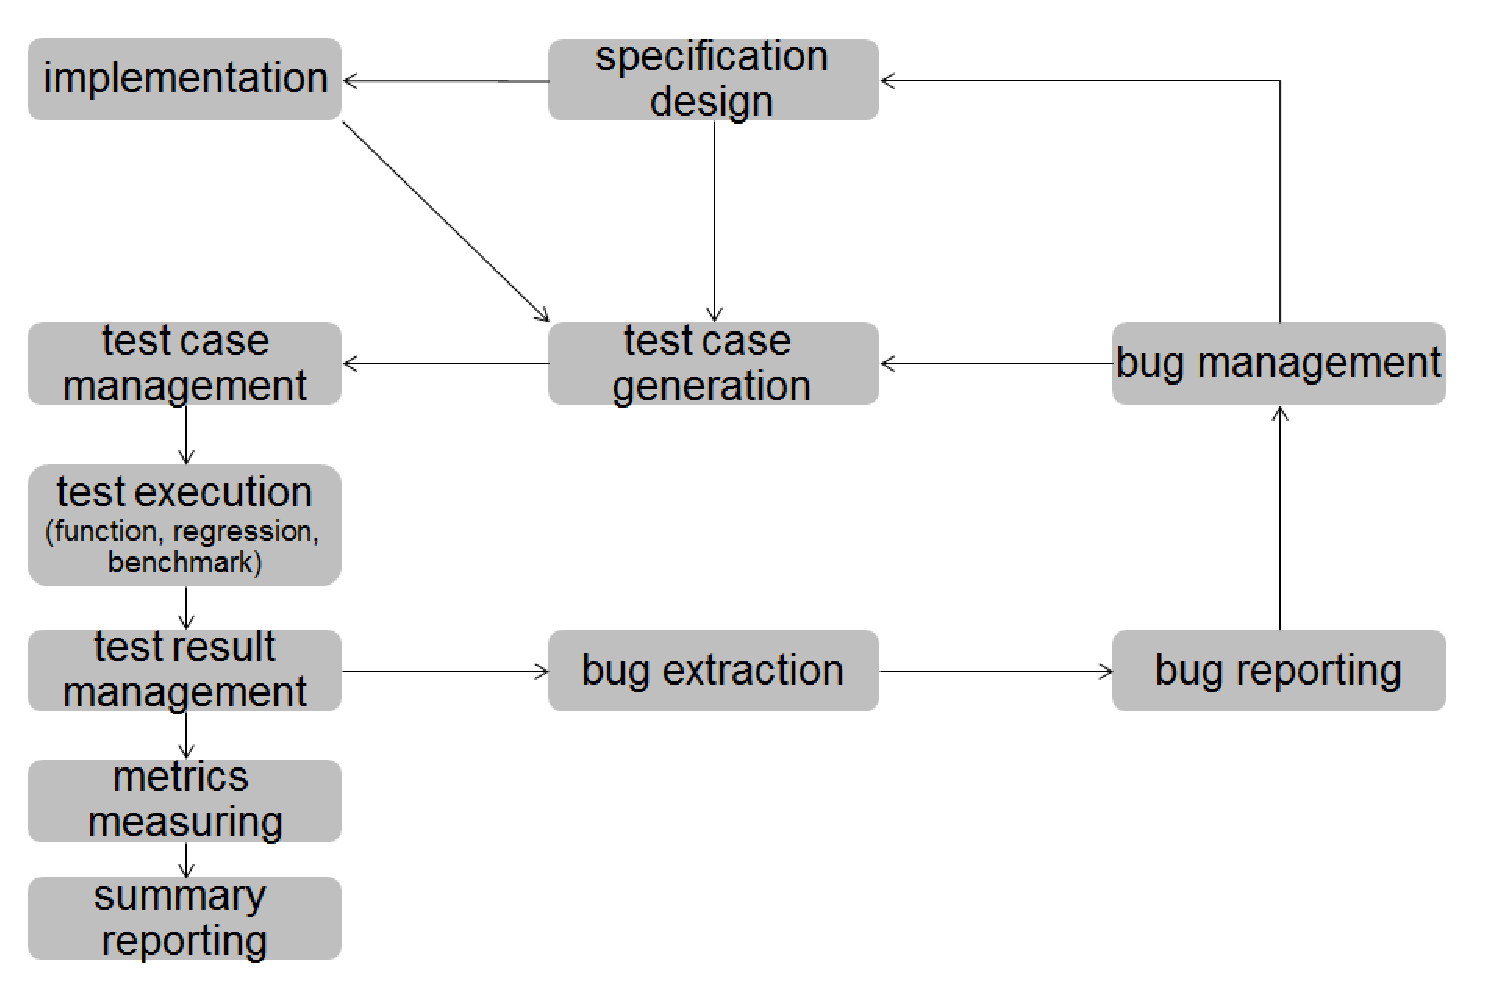
\includegraphics[width=0.8\textwidth]{pic/QA_Tasks.eps}
  \caption{品質管理ライフサイクルを構成する様々なタスク}
  \label{QA_Tasks}
\end{figure}
\par
これらのタスクをサポートするツール類としては、図\ref{QA_Tools}に示すオープンソースの資産が利用可能である。
\begin{figure}[ht]
  \centering
  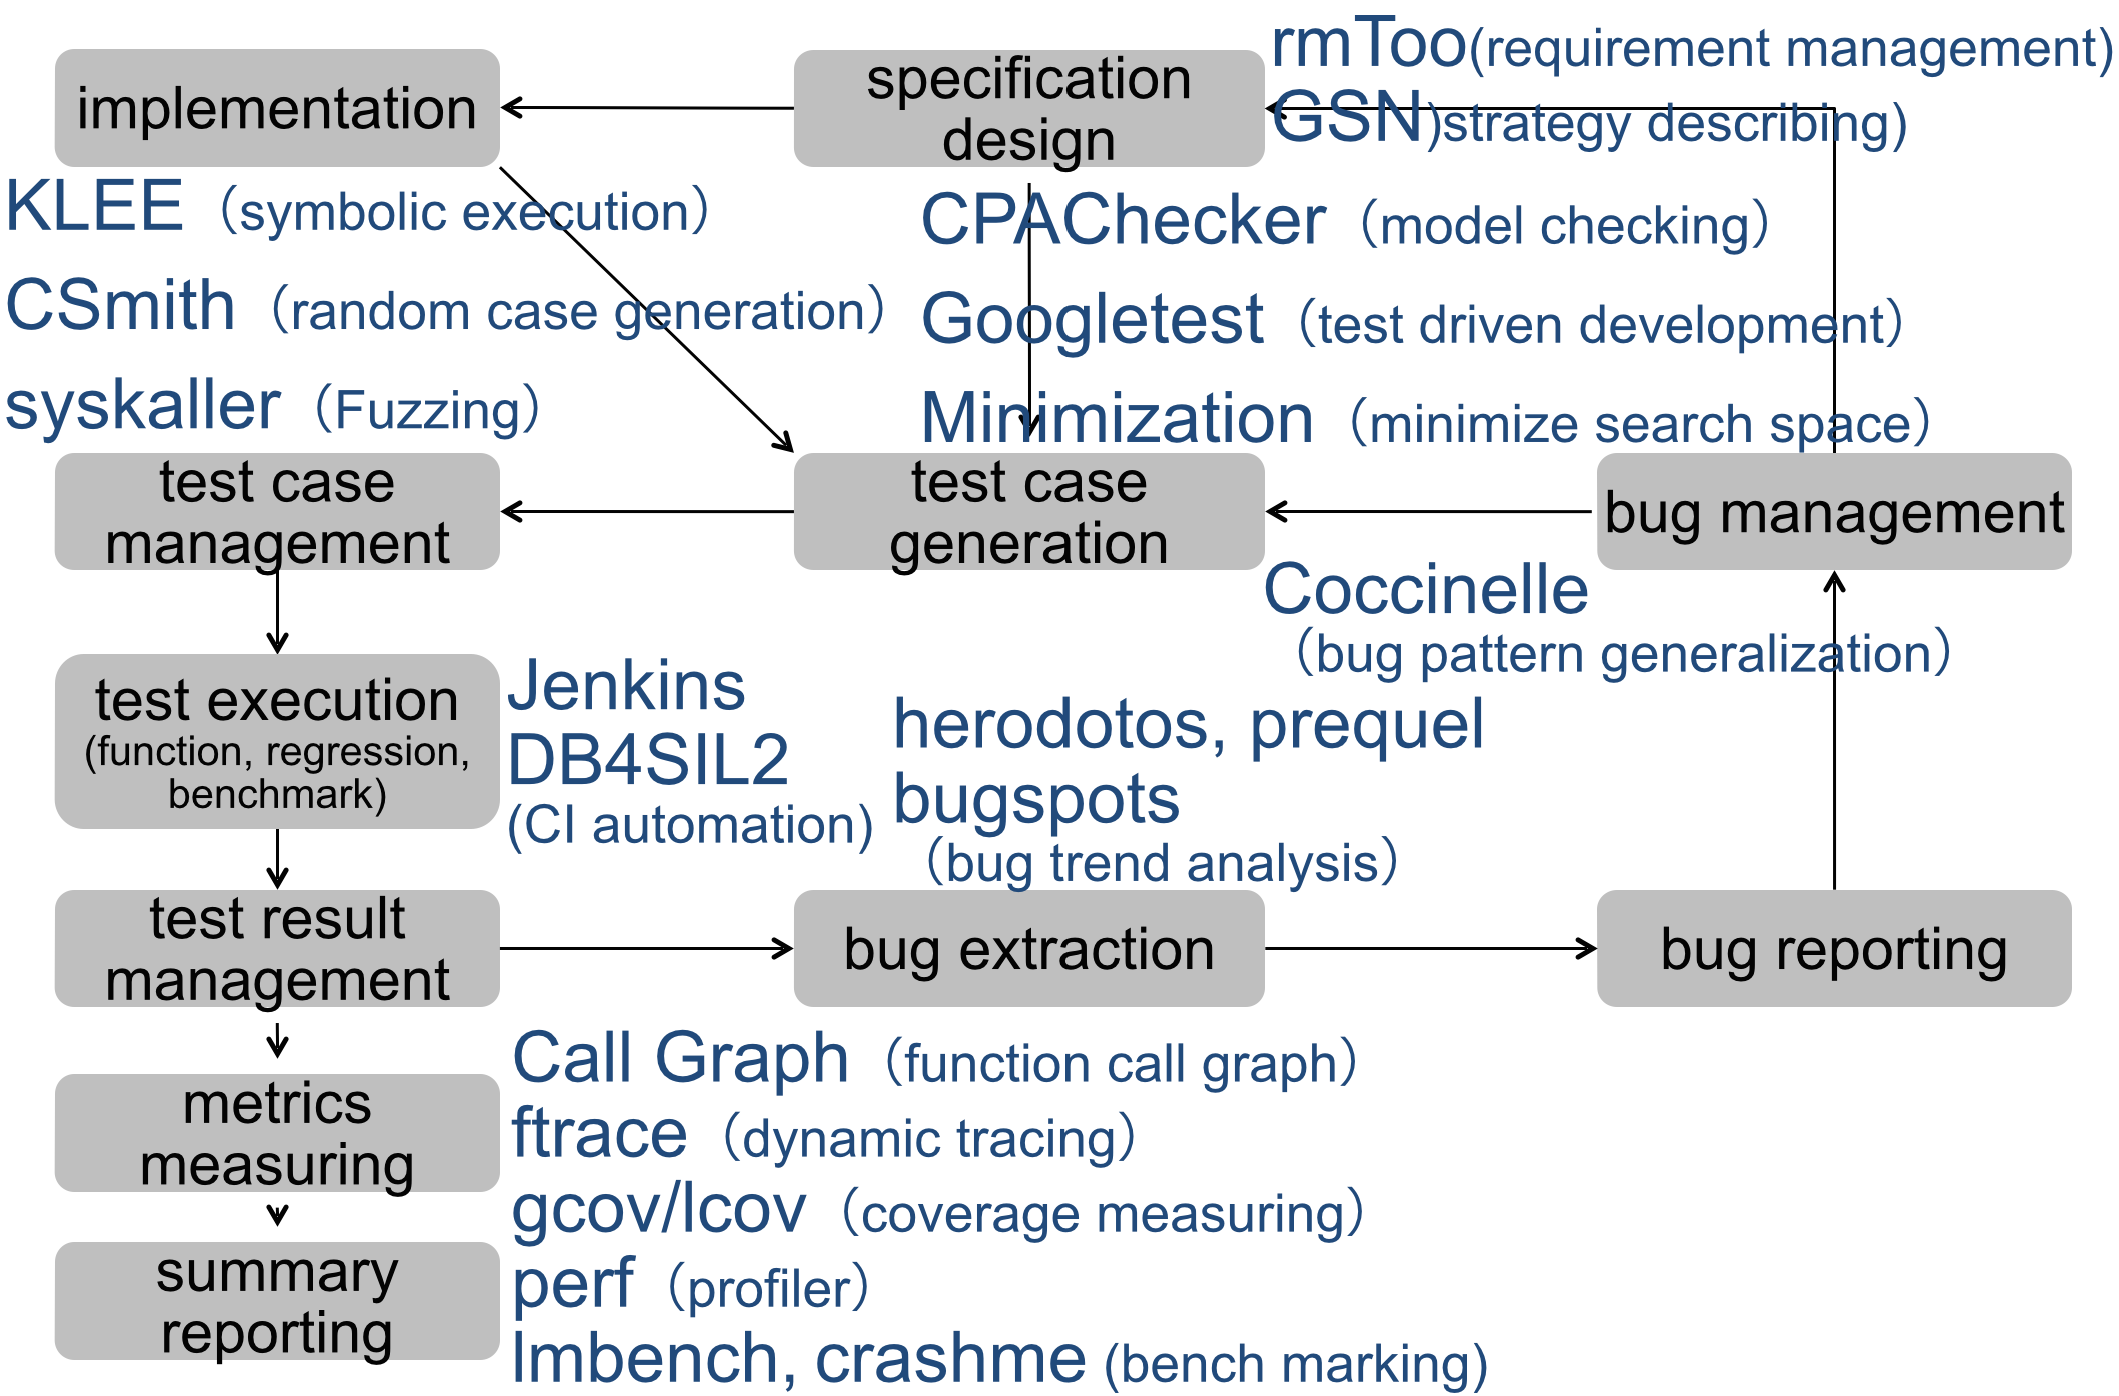
\includegraphics[width=0.8\textwidth]{pic/QA_Tools.eps}
  \caption{品質管理ライフサイクルの各タスクで利用できるツール類の例}
  \label{QA_Tools}
\end{figure}
ただし図\ref{QA_Tools}に示したツール類はあくまでも一例であり、これらのツールを利用すれば各々のタスクを完璧に実施できるという万能なものでもない。
ツールはそれぞれ適用可能なソフトウェアターゲット、得意/不得意な実施内容、実行環境上の制約など様々な性質を持つ。
ツールはあくまでも手段に過ぎず、実際に品質管理ライフサイクルを考える際は「何に対して何を行いたいのか」という目的に対して必要な基準を満たすツール・手法を選定するというアプローチをとることが原則である。
以降は図\ref{QA_Tools}中のツール・手法のうち目的別にいくつかを取り上げそれぞれの調査結果を述べる。

\subsection{バグ検出}
\subsubsection{Coccinelle}
\label{cocci}
\href{http://coccinelle.lip6.fr/}{\acrshort{cocci}} \cite{cocci}はCソースコードのパターンマッチング・変換エンジンである。
例えば、あるAPIを使用している箇所全てについて引数を拡張することや別のAPIに置換するという処理を一括して行うこと、またある論理式・計算式について誤っている表記を一斉に修正すること、さらにC言語の表記を統一するなどコードリファクタリングのような処理を一括して行うことが可能である。
ソースコード中の特定のパターン検索には\acrshort{sm}という非常に柔軟で強力な表現が可能な言語が用いられる。
\acrshort{sm}はスペースや括弧などの表現のばらつきや、変数・関数名の相違などを柔軟に吸収することができ、式の形やデータ構造、処理の流れといったプログラムの意味的な単位に対して作用する。
\acrshort{linux}環境におけるパターンマッチングの技術としては正規表現を使った\verb|sed|コマンドが使われることが多いが、\acrshort{sm}を使った\acrshort{cocci}によるパターンマッチングはそれよりも強力であるという意味で"doped sed"と表現されることがある。
\acrshort{cocci}は"Find once, Fix anywhere"の思想のもとで開発が進められている。
これには、一度\acrshort{sm}でバグパターンを表現してしまえば同種の類似バグを全て改修できる仕組みを作ることで、何度も至る所で同じ修正を繰り返すという無駄な作業を撲滅するという意図が込められている。
\par
\acrshort{cocci} はフランスの研究機関\acrshort{inria}が開発・保守している。
\acrshort{cocci}は関数型言語の\acrshort{ocaml}で書かれており、\acrshort{ocaml}自体も\acrshort{inria}で開発されている。
%\par
\acrshort{cocci}は\acrshort{linux} Kernelのバグ修正に1200件以上の適用実績がある。
\acrshort{cocci}の\acrshort{linux} Kernelにおけるワークフローは、新たに見つかったバグを一般化する形で\acrshort{sm}に書き直して再びソースツリー全体に適用することでその\acrshort{sm}パターンにマッチする同種の残存バグを抽出するというものである。以下に、実際に\acrshort{linux} Kernelに適用実績のある論理演算誤りを修正する\acrshort{sm}の例を示す。
\par
C言語においてnot演算子"\verb|!|"はand演算子"\verb|&|"よりも先に評価されるが、この優先順位関係を誤って認識していたために意図とは異なる論理式を書いてしまう誤りパターンが存在する。
\begin{itembox}[l]{not演算子とand演算子の優先順位を誤った論理演算を含むコード例}
\begin{verbatim}
if(!dma_cntrl & DMA_START_BIT) {
    BCMLOG(BCMLOG_DBG, "Already Stopped\n");
    return BC_STS_SUCCESS;
}
\end{verbatim}
\end{itembox}
\par
この誤りに対して、一般に"\verb|!|式 \verb|&| 定数"のパターンに当てはまるコードを"\verb|!|(式 \verb|&| 定数)"の表記に一括修正する\acrshort{sm}は以下のようになる。
\begin{itembox}[l]{"!式 \& 定数"のパターンを"!(式 \& 定数)"の表記に一括修正する\acrshort{sm}}
\begin{verbatim}
@@
expression E;
constant C;
@@

- !E & C
+ !(E & C)
\end{verbatim}
\end{itembox}
\par
ここで、\verb|@@|で囲まれた箇所はメタ変数宣言部であり、パターンサーチする対象として式(\verb|expression|)、文(\verb|statement|)、型(\verb|type|)、定数(\verb|constant|)、ローカル/グローバル変数(\verb|idexpression|)などを指定することができる。
ここで宣言したメタ変数を使用してパターンの変換ルールを\acrshort{sm}文法に従って表現していく。
この\acrshort{sm}を上記誤りを含むソースファイルに適用すると、\acrshort{cocci}はパターン変換結果を具体的な\verb|diff|形式で出力する。
\begin{itembox}[l]{\acrshort{cocci}によって検出されたパターン変換結果}
\begin{verbatim}
- if(!dma_cntrl & DMA_START_BIT) {
+ if(!(dma_cntrl & DMA_START_BIT)) {
\end{verbatim}
\end{itembox}
\par
\acrshort{cocci}は常にパターンの変換のみを行うものではなく、\acrshort{sm}の書き方によっては\acrshort{cocci}の出力を\verb|diff|形式ではなくパターンマッチしたファイル名と行数のみの表示とするという制御も可能である。
上記のようにして\acrshort{cocci}の出力が得られた後は、それら\acrshort{cocci}の指摘が確かに真のバグであってソースコードに修正を適用するべきものであるかを開発者自身が確認することになる。
ここで\acrshort{sm}の書き方が洗練されていないと、修正する必要のないコードに対しても無駄に\acrshort{cocci}がパターンマッチしてしまい、\acrshort{fp}が大量に出力されてしまうことがある。
\par
これまで実際の\acrshort{linux} Kernel開発でパターン化されバグ修正に貢献実績を持つ\acrshort{sm}が\href{http://coccinellery.org/}{Coccinellery: A gallery of semantic patches} \cite{coccine}で蓄積・公開されている。
Coccinelleryには、式のマクロへの置き換え、API引数追加・削除、API置換、同値表現の統一、デッドロック検出、メモリリーク検出、無効な論理演算検出など\acrshort{linux} Kernel開発で過去にあった既存の修正パターンがほぼ網羅されている。
これらの\acrshort{sm}は再利用することが可能であるが単に使い回せばバグが簡単に検出できるわけではなく、適用する\acrshort{sm}の意図と使い方および期待する出力を各々把握することが必須である。\acrshort{sm}の内容を把握しないまま単に\acrshort{cocci}を実行してもそれらの結果を解釈することができず、また真の指摘が大量の\acrshort{fp}に埋もれてしまうこととなる。
\acrshort{cocci}の\acrshort{fp}に対しては、\href{http://coccinelle.lip6.fr/docs/main_grammar.pdf}{\acrshort{sm}の文法} \cite{sm}に基づいてパターンマッチがより精度よくかつ出力が分かりやすい形となるよう\acrshort{sm}を推敲することが根本的な対策となる。
Coccinelleryに蓄積されている\acrshort{sm}は既に\acrshort{linux} Kernelに適用済みのものであるので、それらを全て再度適用することにはあまり意味がない。
蓄積された\acrshort{sm}の一つの使い方としては、ソースコードに変更を加える前後で\acrshort{cocci}を実行して得られた指摘を\acrshort{fp}含めて比較し、変更前に無く変更後にのみ存在する差分指摘を得ることで回帰テストを効率化する戦略が考えられる。
\par
\acrshort{cocci}は汎用的なセマンティックパターンサーチエンジンであるため、ソースコードのバグ検出以外にも広く様々な使い道が考えられる。
例えばセキュリティ対策としてのコード難読化(code obfuscation)のために、以下のように意味的に等価なコード変換が\acrshort{cocci}で実現できる可能性がある。
\begin{itemize}
  \item 関数名、変数名のランダム文字列への変換
  \item 数値演算、論理演算の等価で複雑な形への変換
  \item 制御構造の複雑化(例:ループ制御の再帰呼び出しへの等価変換)
  \item 関数呼び出し関係の値渡しから参照渡しへ等価変換
  \item データ構造の複雑化(例:構造体の分解または統合)
\end{itemize}
\par
また、\acrshort{cocci}の派生ツールとして、\href{https://github.com/regit/coccigrep}{Coccigrep} \cite{coccigre}というツールがある。
Coccigrepは\acrshort{sm}の文法に基づいてCソースコード中でセマンティック検索するツールで、次のような解析手段を提供する。
\begin{itemize}
  \item 特定の型または特定の構造体の変数がどこで使われているか調べる
  \item 特定の構造体のフィールドがどこで参照されているか調べる
\end{itemize}
\newpage
\subsubsection{Csmith}
\label{compveri}
\href{https://embed.cs.utah.edu/csmith/}{\acrshort{csmith}} \cite{csmith}はCプログラムのランダムジェネレータであり、コンパイラの動作検証を行う目的で使用される。
\acrshort{csmith}は\acrshort{gcc}、\acrshort{llvm}、および商用コンパイラの自動検証とバグ検出に長い実績がある。
特に、コンパイル最適化オプション有効時の誤り検出に顕著な貢献をしてきた。
\par
機能安全対応のソフトウェア開発においては、開発ツール自体についても厳格に採用基準を定め評価を行うことが求められる。
\acrshort{iec61508}-4 3.2.11 において開発ツールは認証対象となるソフトウェアへの影響度に応じてT1, T2, T3の3段階のクラス分けがなされており、そのうちコンパイラはソフトウェア(バイナリ)生成に直接関与するツールとしてT3クラスに分類される。
コンパイラの誤動作は直ちにソフトウェア誤動作の要因となるため、コンパイラの正当性評価には膨大な量のテスト結果と使用実績がエビデンスとして求められる。
実績として十分なエビデンスを得るためには認証対象となるコンパイラについて固定されたバージョンとコンパイルオプションの下、様々な用途の数多くのアプリケーション適用例が必要である(\acrshort{iec61508}-3 7.4.4.2 )。
そのためアプリケーション開発元が単独でコンパイラ認証を行うことは事実上困難であり、機能安全対応のソフトウェア開発には第三者機関によって認証取得済のコンパイラを利用するかまたは専門のコンパイラ評価サービスを利用することが一般的であった。
しかし\acrshort{sil2linuxmp}が対象とするソフトウェアはオープンソースであり、開発ツールも全てオープンソースでなければないという制約があるため、次の2つの理由からコンパイラ検証を第三者に依存することができない。
\begin{itemize}
  \item 認証対象プラットフォームを構成する\acrshort{oss}ソフトウェアのアップデートに依存してコンパイラも持続的なアップデートを前提とするためバージョンを固定できない
  \item コンパイラの検証手法自体もオープンな技術である必要があり、特定の第三者の技術にvendor lock-inされる状態は許容されない
\end{itemize}
\par
以上の制約から、機能安全対応の\acrshort{oss}・\acrshort{linux}プラットフォーム開発で使うコンパイラ検証プロセスは、オープンな技術であり、アップデートにも耐えられるよう検証プロセスが自動化可能で、過去の検証資産を再利用して反復適用できるような性質を持つものである必要がある。
\acrshort{csmith}で生成したエビデンス自体ではコンパイラの正当性を証明するのに十分ではないものの、\acrshort{csmith}は\acrshort{sil2linuxmp}プロジェクトで求められる必要な性質をもつコンパイラ検証ツールとして有効である。
\par
\acrshort{csmith}は次のようなワークフローでコンパイラの正当性検証を行う。
ここでは例として\verb|gcc-4.9|を最適化オプション\verb|-O2|で使用するときの検証方法を挙げる。
\begin{enumerate}
  \item \verb|csmith|コマンドでCプログラムをランダム生成する。
  \begin{itemize}
    \item[] \verb|$ csmith -s <seed> random.c|
  \end{itemize}
  \item 生成したプログラムを検証対象を含む複数のコンパイラにかける
  \begin{itemize}
    \item[] \verb|$ gcc-4.8 -O0 random.c -o random_4.8_O0|
    \item[] \verb|$ gcc-4.9 -O0 random.c -o random_4.9_O0|
    \item[] \verb|$ gcc-4.9 -O2 random.c -o random_4.9_O2|
  \end{itemize}
  \item 生成した複数のバイナリを各々実行し出力結果を比較する
  \begin{itemize}
    \item[] \verb|$ ./random_4.8_O0|\\\verb|checksum = 54A570D1| $\cdots$\verb|gcc-4.8|の\verb|-O0|でコンパイルしたバイナリの実行結果
    \item[] \verb|$ ./random_4.9_O0|\\\verb|checksum = 54A570D1| $\cdots$\verb|gcc-4.9|の\verb|-O0|でコンパイルしたバイナリの実行結果
    \item[] \verb|$ ./random_4.9_O2|\\\verb|checksum = 54A570D1| $\cdots$\verb|gcc-4.9|の\verb|-O2|でコンパイルしたバイナリの実行結果
  \end{itemize}
\end{enumerate}
\par
全ての実行結果の出力(\verb|checksum|値)が一致すれば、ここでランダムに生成したプログラム\verb|random.c|に関する検証は成功である。
もしいずれかの結果が他と異なる出力となる、またはバイナリ実行が失敗する、またはコンパイル自体が失敗する場合は、その事象を該当コンパイラおよびオプションの組合せに関するバグとして調査する。
以上の手続きを、\verb|csmith|で生成するランダムCプログラムの種を変えながら繰り返し実施し続ける。
検証成功したランダムプログラム数が増えるほど、その実績がそのコンパイラとオプションの組み合わせに対する品質を保証するエビデンスとなる。
\par
\acrshort{csmith}が生成するランダムプログラムがコンパイラの正当性を示すために十分に有効なテストケースとなるためには、そのプログラムがC言語で表現可能な出来る限り多様なコードを含んでいなければならない。
しかしこの要件は、コンパイラのテストケースとして使われるプログラム
%\acrshort{csmith}でランダム生成したプログラム(コンパイラテストケース)
はC言語仕様で不定または未定義の振る舞いをするコードを含んでいてはいけないという制約とトレードオフの関係にある。
例えば、\verb|a = f(b) + g(b)|という式について\verb|f(b)|と\verb|g(b)|のどちらが先に評価されるかは不定である。\verb|f(b)|と\verb|g(b)|が共に\verb|b|を変更するとき、コンパイラの実装によっては\verb|f(b)|と\verb|g(b)|の評価順序が逆転してその結果式全体の評価結果\verb|a|が異なる可能性があるが、この挙動はC言語仕様では不定であるのでどちらの挙動も正しい。
また、ゼロ除算、$-1$での剰余、配列領域外アクセス、NULLポインタ開放、整数オーバーフロー、未初期化変数の参照などC言語仕様上未定義の動作となるコードは、コンパイラによっては気を利かせた挙動をするものがあるものの、ほとんどの場合はプログラムがクラッシュする結果となるため有効なテストケースとならない。
このように、コンパイラの正当性検証テストケースとしてはC言語仕様で厳密に定義された振る舞いをするコードのみからなるプログラムを使用しないと、上記の\acrshort{csmith}のワークフローでは\acrshort{fp}が大量に生成されてしまう。
\par
このため、\acrshort{csmith}のアルゴリズム開発では当初から現在まで「不定または未定義挙動のコードを含まずコンパイルエラーにならにコードで可能な表現を多く含むランダムプログラム生成」をいかに正確に実現するかに努力が払われてきた。
生成される\acrshort{fp}には不定/未定義挙動が原因であるものと既知問題であるものがあり、真のバグ選別および有効なバグレポートの作成がとても困難であるという経験から、\acrshort{csmith}を使ったコンパイラ検証プロセスの自動化とバグトリアージ(\acrshort{fp}の山から真の指摘を抽出する)方法の開発が課題であるとされている。
これまで\acrshort{csmith}が適用された実績がある\acrshort{gcc}はごく一部のバージョンとオプションの組合せに対してのみであり、\acrshort{gcc}のアップデートに対して最新のバージョンと最適化オプションの組合せ検証網羅および\acrshort{csmith}による検証作業が追いついていない状況である。
また\acrshort{csmith}による検証自体をどこまでやれば十分であるかを一様に判断することが困難である。機能安全対応の際は、例えば蓄積されたテスト結果を用いて「統計的に残存バグがあと何件以下」というような論理的な根拠を構築して認証機関に十分性を示すことが求められる。
\subsection{テストケース生成}
\subsubsection{KLEE}
\label{klee}
\href{https://klee.github.io/}{\acrshort{klee}} \cite{klee}は\acrshort{se}ツールの一種で、既存のソースコードを元に同値分割テストケースを自動生成する目的で使用できる。
\acrshort{klee}は与えられたCソースコードから可能な実行パスに遷移するための引数や変数の状態組合せを探索して模擬実行する(\acrshort{se})。
以下に\acrshort{klee}がCソースコードを元にテストケースを生成する挙動の例を示す。
\begin{itembox}[l]{テスト対象関数の例}
\begin{verbatim}
int get_sign(int x) {
  if(x == 0)
    return 0;

  if(x < 0)
    return -1;
  else
    return 1;
}
\end{verbatim}
\end{itembox}
\par
上記関数に対して\acrshort{klee}は以下のように振る舞う。
\begin{enumerate}
  \item 関数中の全分岐(\verb|if-else|)を特定する
  \item 特定した各分岐に遷移するための変数\verb|x|の条件を探索する
  \item 探索した各条件について具体的な代表値を一組決める
\end{enumerate}
\par
この結果3パターンの\verb|x |$ = \{0, 16843009 (> 0), -2147483648 (< 0)\}$で\verb|get_sign()|を呼ぶテストケースが生成される。
生成された3つのテストケースはそのまま何度でも再利用できるため例えば回帰テストへの応用が考えられる。
\par
\acrshort{iec61508}は同値分割テストケース生成について仕様に基づく方法とプログラムの内部構造に基づく方法の2通りを示唆しており(\acrshort{iec61508}-7 Ed2 C.5.7)、このうち\acrshort{klee}はプログラムの内部構造からテストケースを生成するツールとして適用できる。
\acrshort{klee}ではソースコードがあればテスト対象の仕様を特に知らなくてもテストケース生成が可能であるが、関数引数をシンボリック変数にしてテスト対象を呼び出すためのテストドライバの作成は必要となる。
\par
\acrshort{klee}のアルゴリズムはヒューリスティック探索に基づくため100\%分岐網羅を保証するものではない。
上記の例のように単純なプログラムであれば100\%分岐網羅を達成することができるが、実用上の大きなプログラムでは計算コスト上の制約が問題となる。
\acrshort{klee}のパフォーマンスを向上させるためには、例えば無駄な探索をさせないようにシンボリック変数の動く範囲を指定することが有効である。
テスト対象となる関数の引数が数値ならばその上限と下限を、文字列ならば各文字が取り得る値を、または論理式を使い複数の引数の制約関係を表現することもできる。
これを利用すれば、シンボリック変数の条件をテストドライバ側で指定することで入力仕様に基づいたテストケースを設計することができる。
また、用意された4種類の探索アルゴリズムから適当なものを選択したり、アルゴリズムをラウンドロビンで組合せたり、最大探索深さやタイムアウト時間の設定ができたり、優先して探索するシンボリック変数の条件が指定できるなど探索戦略を柔軟に調整する手段が提供されている。
\par
\acrshort{klee}は\acrshort{llvm}プラットフォーム上で動作するため、\acrshort{llvm} bitcodeにコンパイルできないプログラムには\acrshort{klee}が適用できないという制約が存在する。
\acrshort{sil2linuxmp}では\acrshort{bb}に対して\acrshort{klee}を使用してテストケース生成と同値分割テストを実施することが検討されている。
\acrshort{klee}はその性質上、プログラムの挙動が入力のみに依存して決定的であるものに対して有効で、外部からの割り込み、並列実行、タイミング等が挙動に影響する対象は適用が困難である。そのため\acrshort{linux} Kernelに対しては\acrshort{klee}による解析は適さない。
%\subsubsection{Syskaller}
\subsection{反例検出}
\subsubsection{CPAChecker}
\href{http://cpachecker.sosy-lab.org/}{\acrshort{cpa}} \cite{cpa}はCプログラムの各コードブロックへの到達可能性を検証するモデルチェックツールである。
Cソースコードを入力として制御フローオートマトンを導出し、予め定義されたエラー状態へ遷移する可能性を解析する(図\ref{cpa})。
CPAは"Configurable Program Analysis"の頭文字であり、数あるプログラム状態遷移解析ツールの中でも、設定次第で一つのツールで複数用途の解析に使用可能であることが特徴である。
例えば、メモリアクセス違反など特定の動的挙動に絞って解析を行う場合や、仕様検証のために正確性を重視したモデルチェックを行う場合などで、計算資源と正確性のトレードオフを考慮してメモリ割り当て量やタイムアウト時間などを制御することや、検証項目によってアルゴリズムを選択することができる。
これらの検証アルゴリズム・パラメータセットは予め用意された設定が180存在しており、目的に従って既存の設定を選択使用することができる。
\acrshort{cpa}はLinux Driver Verification Project (linuxtesting.org)で採用されており、Linuxデバイスドライバに対して150件以上のバグ修正実績がある。
\begin{figure}[ht]
  \centering
  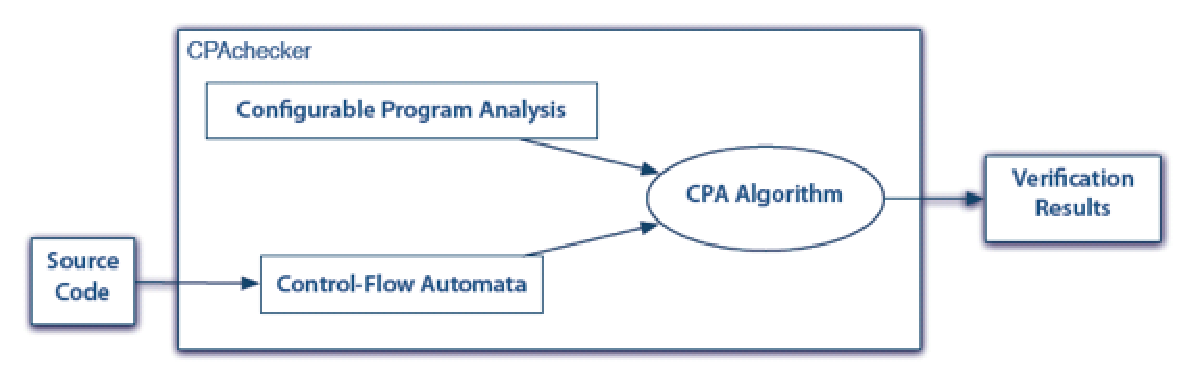
\includegraphics[width=\textwidth]{pic/cpa.eps}
  \caption{\acrshort{cpa}のワークフロー}
  \label{cpa}
\end{figure}
\par
以下に、プログラムのエラー状態への遷移可能性を\acrshort{cpa}によって解析する例を示す。
\begin{itembox}[l]{定義されたエラー状態に到達し得るミスがあるコード例}
\begin{verbatim}
#include <stdio.h>

int main(void) {

  double x, y;

  // xで受け取った実数の絶対値をyに入れる
  scanf(“%lf”, &x);
  // 負数かどうかの判定を誤って-1以下の条件としてしまった実装
  y = (x <= -1) ? (-1) * x : x;

  printf(“abs(%lf) = %lf\n”, x, y);

  // 計算した絶対値が非負でなかったらエラーとする
  if(y < 0) {
    goto ERROR;
  }

  return 0;

// CPACheckerはソース中の”ERROR”ラベルかasseart()を見つけて
// そこへ遷移する条件(反例)を探す。このケースでは”ERROR”ラベルの代わりに
// asseart(y < 0); としても同じ検証ができる。
ERROR:
  return 1;
}
\end{verbatim}
\end{itembox}
\par
\acrshort{cpa}はこのプログラムファイルと検証アルゴリズムの設定およびパラメータセットを読み込んで、検出されたエラー状態に遷移するための変数の状態を探索する。
出力はには、\acrshort{gv}フォーマット(.dot)による\acrshort{cfa}と\acrshort{art}が含まれる。
\acrshort{cpa}の結果はReport Generatorによりwebブラウザで視覚的に表示できる形式で出力することが可能である(図\ref{cpareport})。
\begin{figure}[ht]
  \centering
  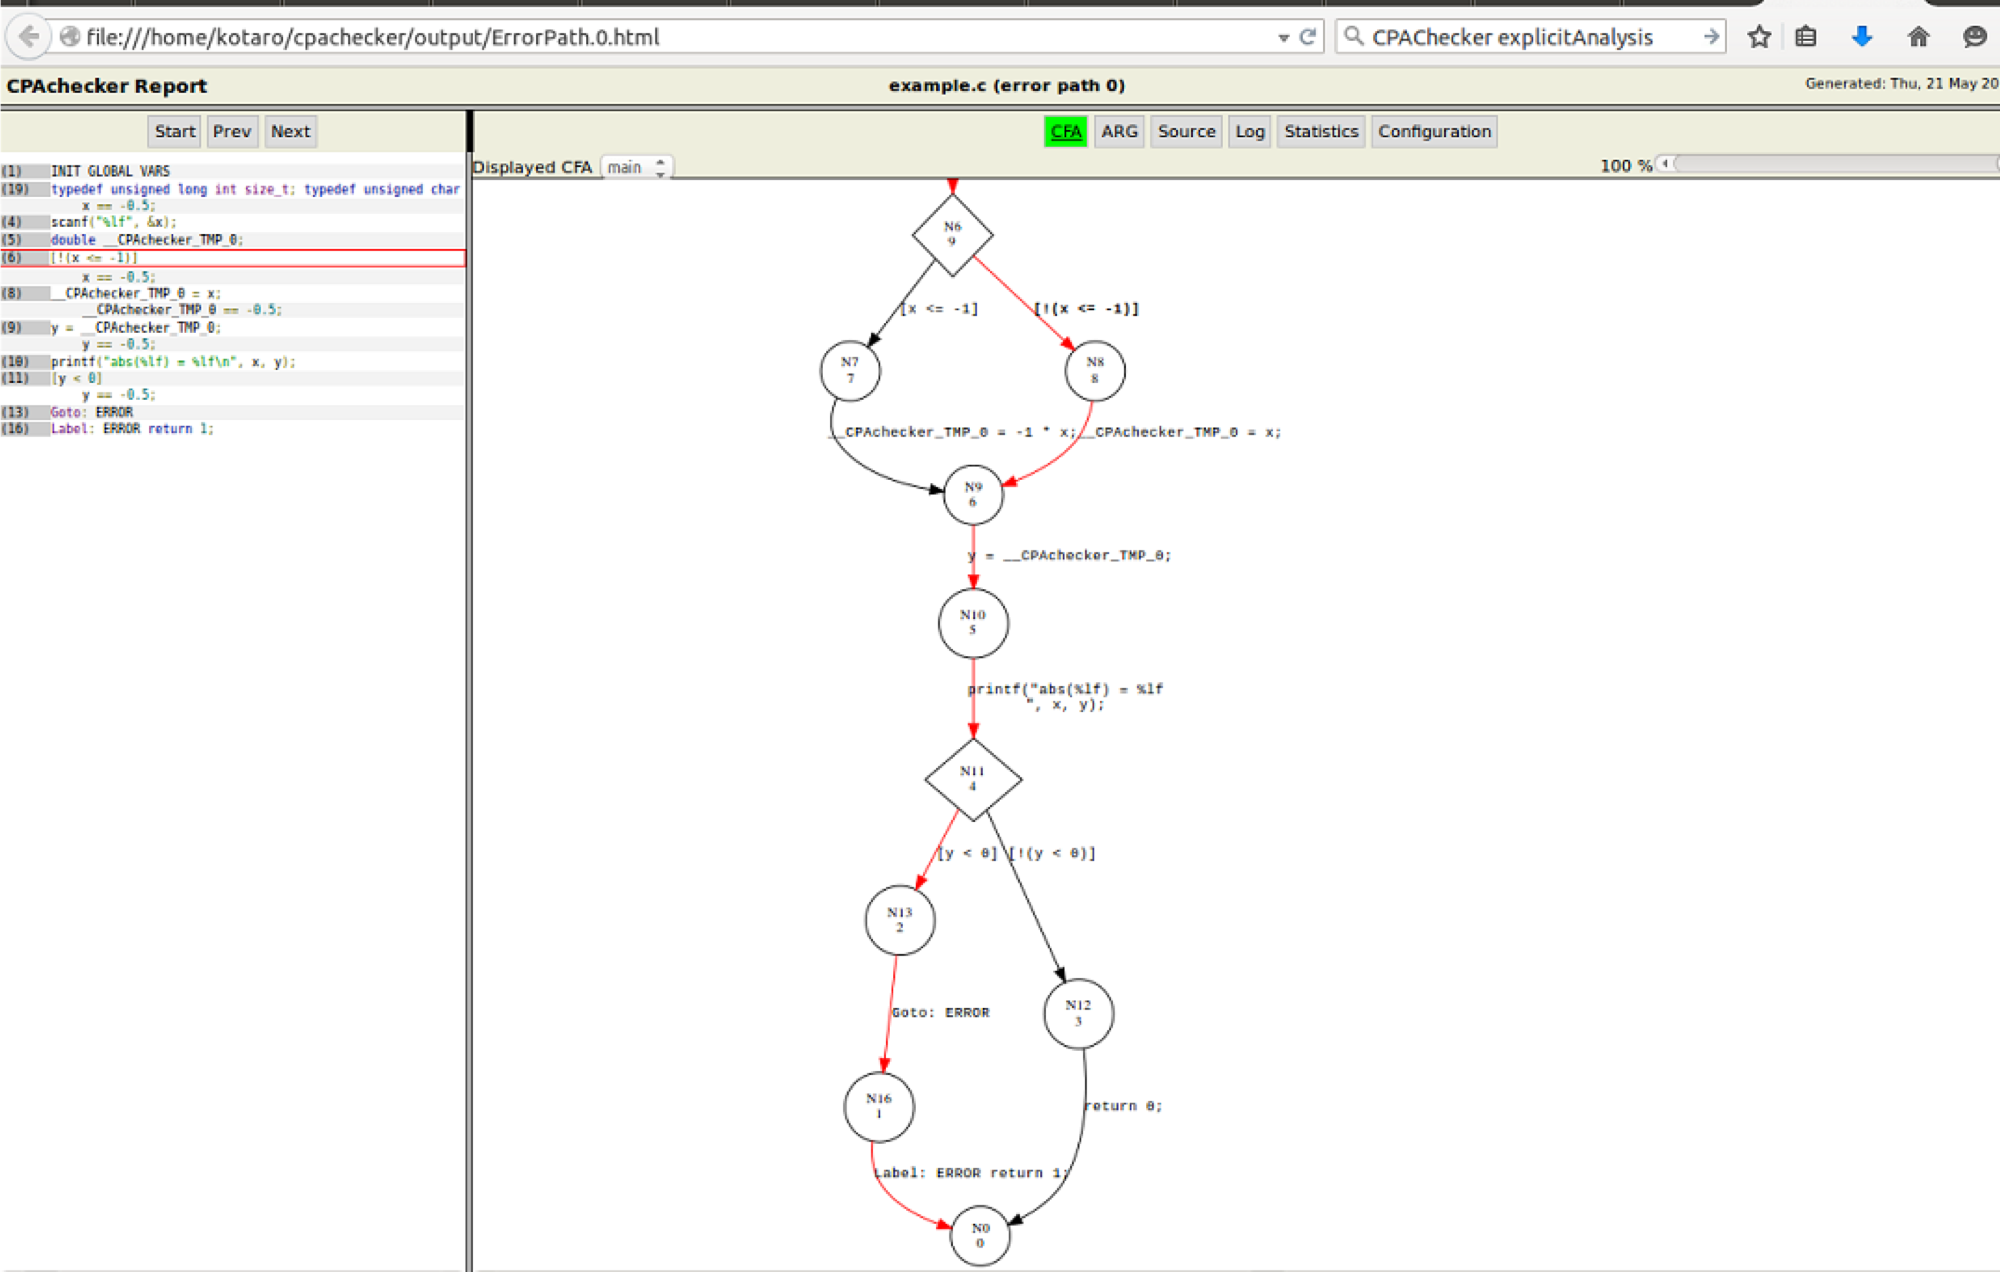
\includegraphics[width=\textwidth]{pic/cpareport.eps}
  \caption{\acrshort{cpa} Report Generatorの出力例}
  \label{cpareport}
\end{figure}
\par
図\ref{cpareport}のReport Genetatorの出力右半分には関数毎の状態遷移図を表す\acrshort{cfa}が表示されており、各エッジやノードをクリックすると該当する制御文や宣言などのコードにジャンプすることができる。
ここで、検出されたエラーパスは赤く表示されており、このパスを通る際のコールスタックがレポートの左半分に表示されている。
コールスタックの各行からも、該当する\acrshort{cfa}のエッジまたはノードにジャンプすることができる。
図\ref{cpareport}の左画面(6)の次の行に表示されている\verb|x == -0.5|が、探索された反例(Counter Example)の具体値であり、これによってこのプログラムは\verb|x == -0.5|のときに\verb|ERROR:|ブロックに遷移しプログラムが異常停止することが分かる。
\par
以上の使用例に代表されるように、\acrshort{cpa}は予め定義されたエラー状態に到達し得るかどうかの判定(Reachability Analysis)と、エラー状態に遷移し得る場合はその条件(Counter Example)を具体的な変数状態で探索する。
また検証アルゴリズムの設定によっては、NULLポインタアクセスやバッファオーバーフローなどのメモリアクセス違反が発生し得るかどうかの判定も可能である。
予めエラー状態がコード中に定義されていればそこに遷移する条件を自動的に検出できることから、\acrshort{gt}等のテスト駆動開発手法と上手に併用出来れば強力な回帰テストフレームワークを構築できる可能性がある。
\par
\acrshort{cpa}が適用可能なC言語表現は、ループ、配列、条件分岐、ポインタ、ヒープ、再帰、浮動小数点表示等と幅広く、\acrshort{cpa}は特に制御フローとメモリアクセスの安全性解析を得意とする。
一方で、深くネストされたループやメモリを大量に消費する再帰構造を持つフローの解析は得意でなく、\acrshort{cpa}は無限ループの検出やデッドロックの検出を行うことができない。
また、マルチスレッド等の並列実行構造を持つフローの解析にも対応していない。
図\ref{svcomp}は、2015年に行われた国際的なソフトウェア検証コンペティション\href{http://sv-comp.sosy-lab.org/2015/results/index.php}{\gls{sv}の総合結果} \cite{sv}である。
\acrshort{sv}では様々な種類の検証課題に対して各々検証プラグラムのベンチマークが測定される。
\begin{figure}[ht]
  \centering
  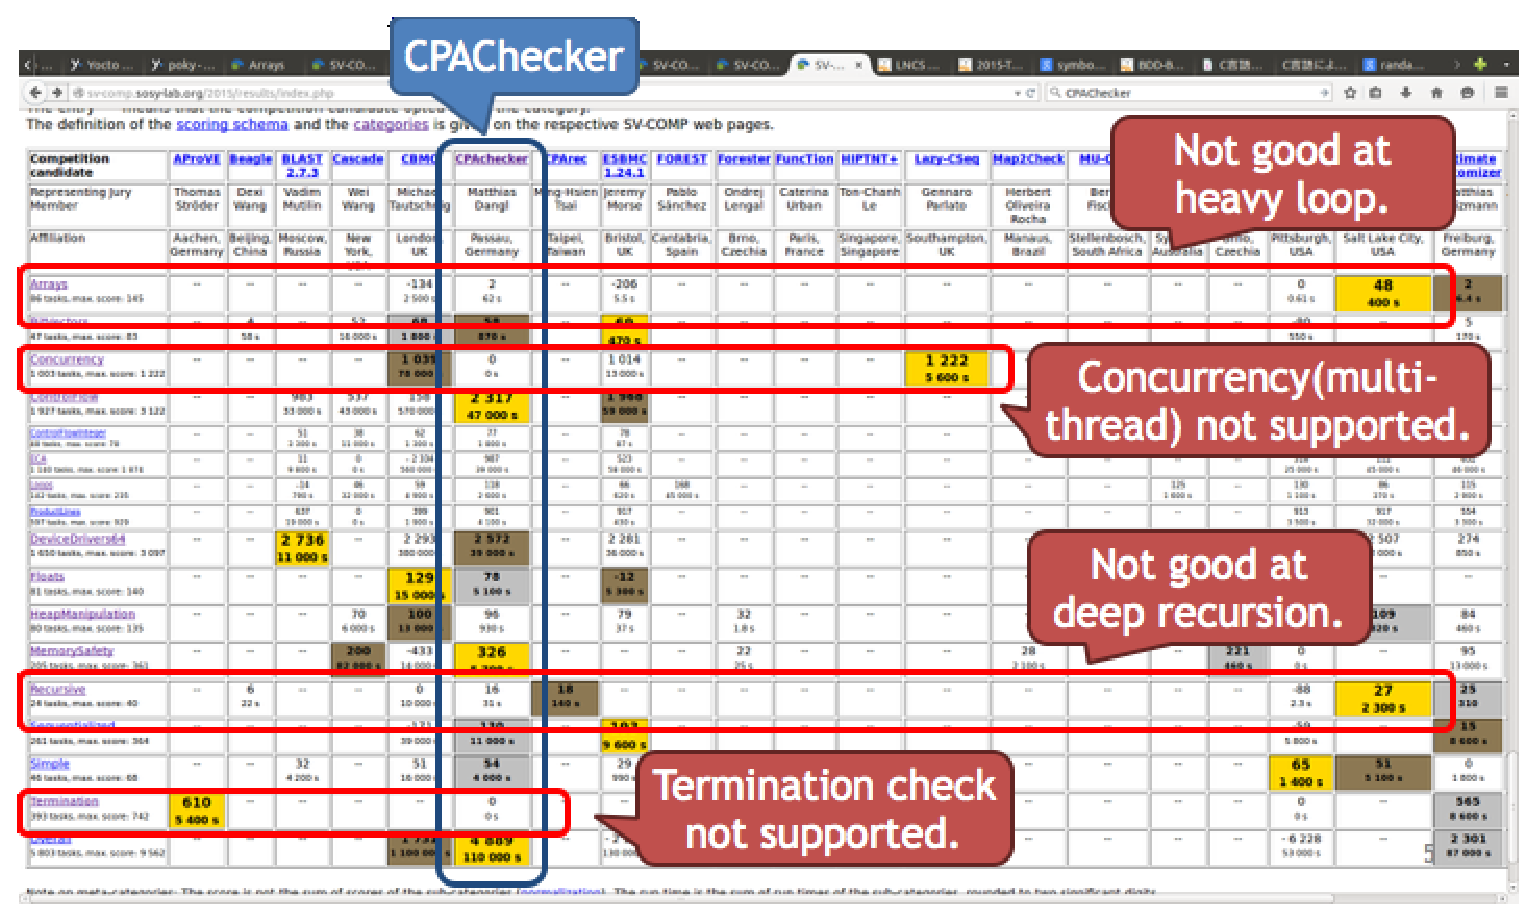
\includegraphics[width=\textwidth]{pic/svcomp.eps}
  \caption{\gls{sv}2015 の総合結果}
  \label{svcomp}
\end{figure}
\par
\acrshort{cpa}は制御フローやメモリアクセスの安全性解析および\acrshort{linux}デバイスドライバの解析で圧倒的なパフォーマンスを示しており総合評価でもトップの成績を残している。
ただし、先述したように深いループ・再帰の解析は不得意で停止性検証および並列実行の解析は対応していないため、これらの検証課題に対しては他のツールが優位となっている。
例えばプログラムの停止性検証(termination check)では\href{http://aprove.informatik.rwth-aachen.de}{\gls{aprove}} \cite{aprove}という停止性検証に特化した強力なツールが存在し、実際のデバイスドライバの検証にも大きな貢献をしてきている。
停止性検証は古くから研究されている問題で、制御フローの解析問題とは独立にその分野自体に長い蓄積がある。
全ての問題に対応する万能なツールを追求することは本質的ではなく、あくまでも目的とする検証対象に合致したツール・手法を選択しそれらの制約をよく把握した上で適切なツール・手法を使用することが重要である。
\subsection{メトリクス測定}
\subsubsection{CodeViz}
\label{cv}
\href{http://www.csn.ul.ie/~mel/projects/codeviz/}{\acrshort{cv}} \cite{cv}はC/C++プログラムの関数呼び出し関係を視覚化する関数コールグラフ生成ツールである。
\acrshort{sil2linuxmp}では動的トレーシングツールの結果と組み合わせて呼び出し関係のカバレッジを測定する用途で使用することが検討されている(詳細は\ref{callgraph}項で記載)。
関数コールグラフ生成ツールは、ソースコードを静的に解析してグラフを得るものと、実際にプログラムを動かしたときの挙動から動的にグラフを得るものとに大別できる。
このうち\acrshort{cv}は静的に関数コールグラフを生成するツールである。
静的コールグラフ生成ツールとしては他に\acrshort{gnu}プロジェクトの\acrshort{cflow}がある。
\acrshort{cflow}と比較して、\acrshort{cv}は関数ポインタを介した関数呼び出し関係も出力に反映できるという利点がある。
図\ref{vfs}は、\acrshort{linux} Kernel 4.3.3ツリーの\verb|fs/read_write.c|に対して\verb|vfs_read()|関数から先のコールグラフを生成した例である。
\begin{figure}[ht]
  \centering
  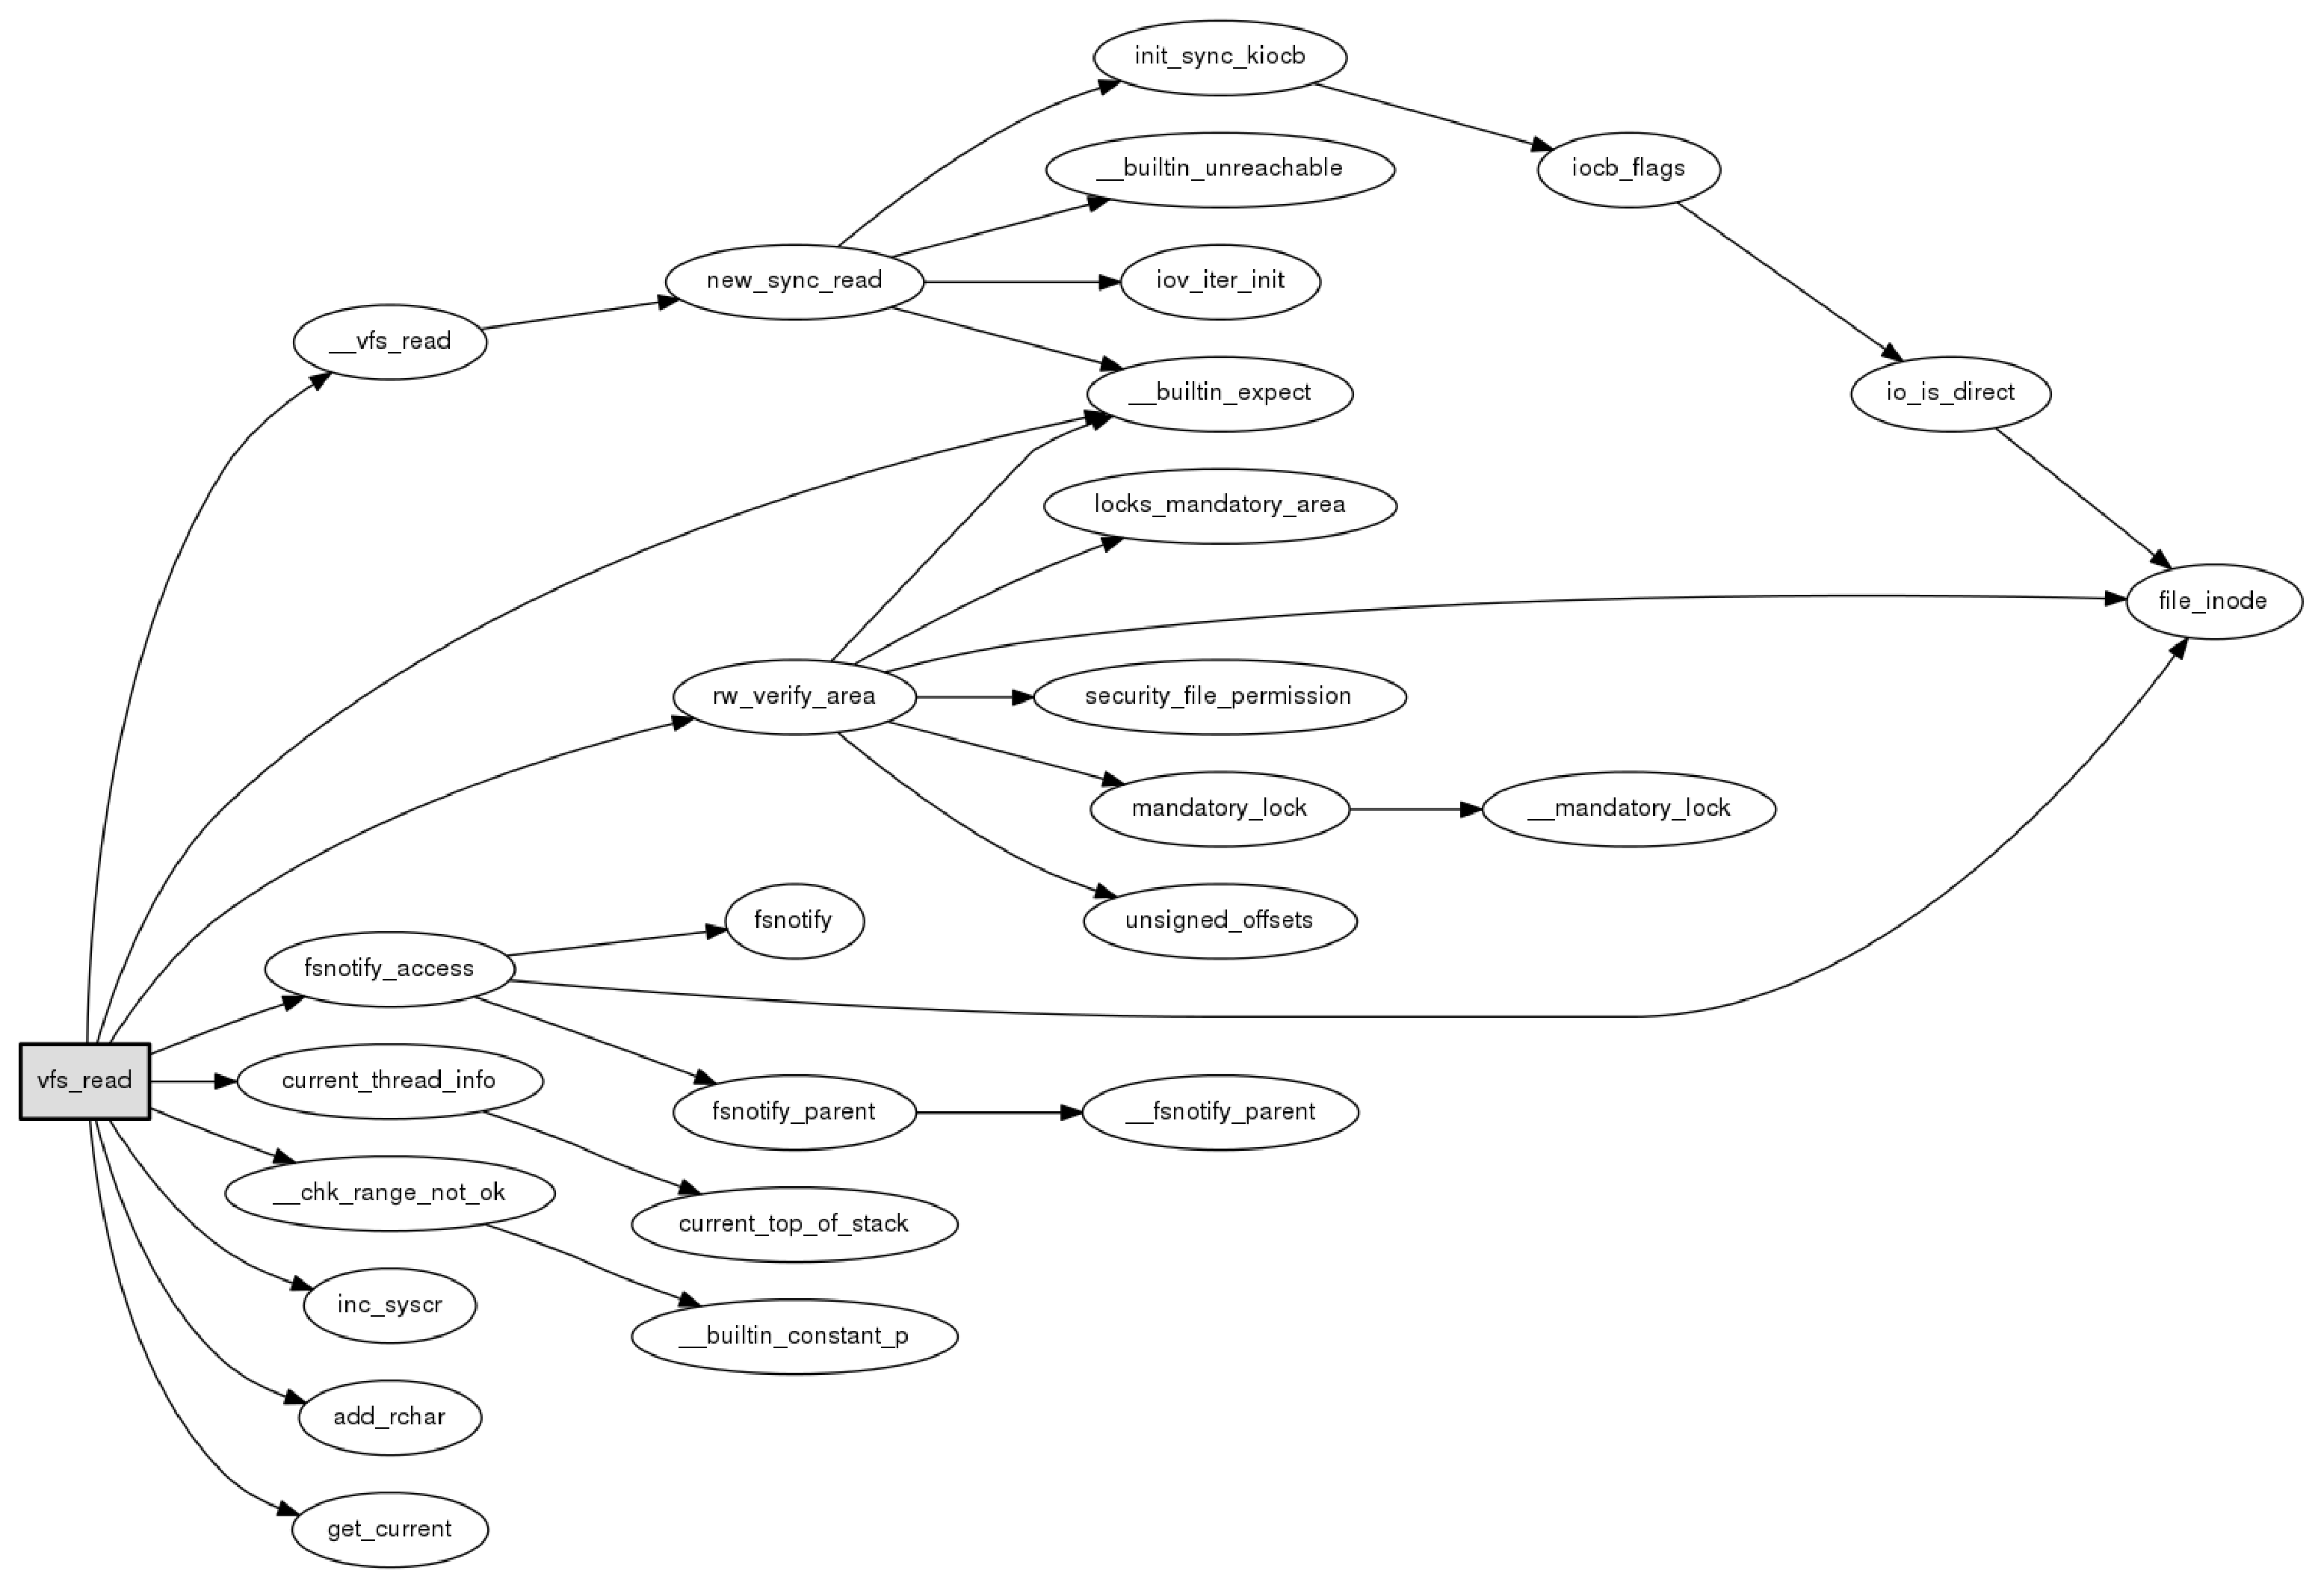
\includegraphics[width=0.8\textwidth]{pic/vfs_read.eps}
  \caption{\acrshort{linux} Kernel fs/read\_write.cのvfs\_read()関数コールグラフを\acrshort{cv}で生成した例}
  \label{vfs}
\end{figure}
\par
\acrshort{cflow}と比較して、\acrshort{cv}の出力は次の点でより洗練されたものとなっている。
\begin{itemize}
  \label{cv_vs_cflow}
  \item \verb|vfs_read()|と\verb|__vfs_read()|を区別する(\acrshort{cflow}は\verb|__|接頭辞が無視され両者が同一ノードになってしまう)。
  \item 意図しないマクロ\verb|likely()|や\verb|unlikely()|のコールグラフへの出現が抑制されている(\acrshort{cflow}では関数ノードとして出現してしまう)。
  \item \verb|loff_t|など独自定義の型名が正しく処理されている(\acrshort{cflow}では誤って\verb|loff_t|が関数ノードとして出現してしまう)。
\end{itemize}
\par
\acrshort{cv}は、コールグラフデータの生成手段としてdepnとnccという二つの方法を提供している。
depnは特定の\acrshort{gcc}のバージョン(3.4.6か4.6.2)に対して専用のパッチを当てたものを使用してコールグラフデータを生成するため手順がやや複雑である。
\href{http://students.ceid.upatras.gr/~sxanth/ncc/}{ncc} \cite{ncc}は特に\acrshort{gcc}に対するパッチは必要なく手順が簡単である上、関数ポインタを介した呼び出し関係も表現することができる利点がある。
\acrshort{sil2linuxmp}では、手順の簡易さと関数ポインタを扱えるという利点からnccを利用する検討が進んでいる。
nccはソースコードのブラウジング用途に開発されたコンパイラである。
なお、グラフデータの視覚化は\acrshort{cv}付属のツールを用いて画像を生成する方法と、nccパッケージに付属する\acrshort{gv}データ(.dot)変換ツールを用いる方法がある。
関数コールグラフを利用した呼び出し関係のカバレッジメトリクス測定として\acrshort{sil2linuxmp}で検討されている方法については\ref{callgraph}項で記載する。
%\subsubsection{ftrace}
\newpage
\subsubsection{syzkaller}
\href{https://github.com/google/syzkaller}{\acrshort{syzkaller}} \cite{syzkaller}は、\acrshort{linux} Kernelシステムコールに対する\acrshort{fuzzer}プログラムである。
Fuzzerとは、大量のランダムデータ・ランダムテストケースを生成・実行することで検査対象プログラムのミスや脆弱性を見つけるテストプログラムの総称を言う。
\ref{klee}項で触れた\acrshort{csmith}はコンパイラに対する\acrshort{fuzzer}である。
\acrshort{syzkaller}はシステムコールに対するカバレッジを指標にテストケースを自動生成・実行する。
これを利用すると、ターゲットシステムの\verb|debugfs|からシステムコールに対するテストカバレッジ情報を取得できたり、クラッシュ情報やテスト結果を取り出して開発ホスト側のwebインタフェースでサマリを表示したりということが可能になる(図\ref{syzkaller})。
\begin{figure}[ht]
  \centering
  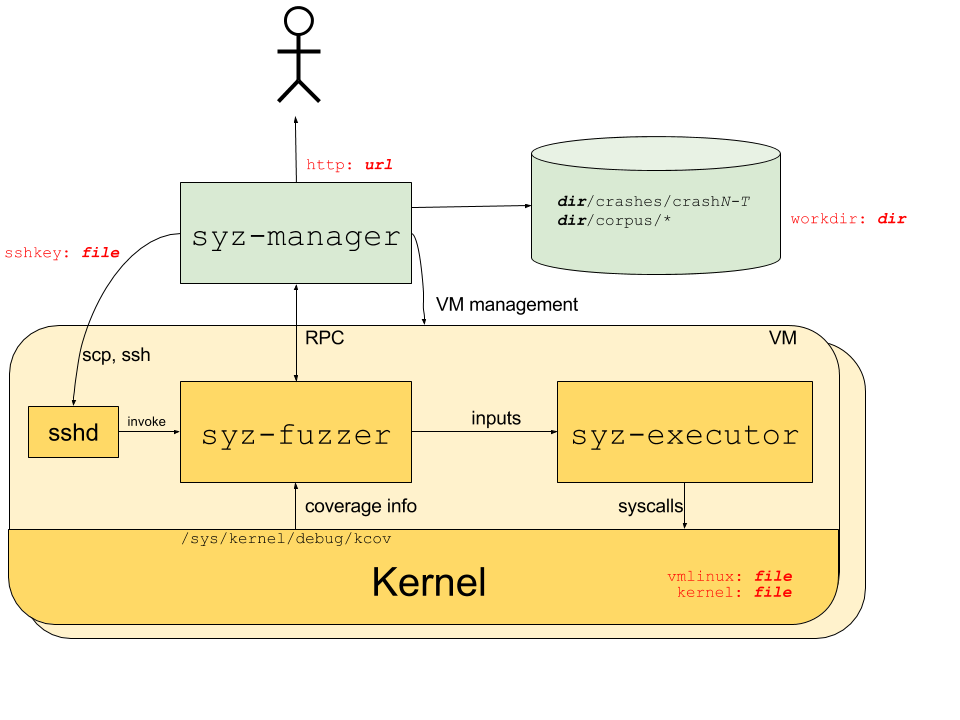
\includegraphics[width=0.8\textwidth]{pic/syzkaller.eps}
  \caption{\acrshort{syzkaller}システムの全体アーキテクチャ}
  \label{syzkaller}
\end{figure}
\par
\acrshort{syzkaller}は2015年10月に開発が始まった新しいプロジェクトであるため成熟度は十分でなく、現在サポートされるプラットフォームは\acrshort{qemu}のみで他の仮想マシンや物理ターゲットボードは未サポートである。
また現状は導入の前提条件として最新の\acrshort{gcc}を自前でビルドする必要があったり、\acrshort{linux} Kernelに特別にパッチを当てる必要があったりと手順に難がある。
\acrshort{sil2linuxmp}では\acrshort{linux} Kernelシステムコールのテストカバレッジ向上とメトリクス測定のために\acrshort{syzkaller}利用すること想定して調査が継続されている。
\subsection{バグ選別}
\ref{cocci}項で述べた通り、\acrshort{cocci}はそれ単独で用いると大量の\acrshort{fp}を生成してしまうため、真のバグをいかに選別するかが効率的なバグ検出にとって重要となる。
\subsubsection{Herodotos}
\href{http://coccinelle.lip6.fr/herodotos/docs/herodotos.html}{\acrshort{hero}} \cite{hero}は、\acrshort{cocci}の\acrshort{fp}を抑制する目的で\acrshort{cocci}と同じ\acrshort{inria}が開発しているツールで、特定のバグパターンの出現傾向を世代間にわたって解析することができる。
\acrshort{sm}で一般化したバグパターン各々についてバグのトレンドと残存期間などを視覚化することで、そのプロジェクトの開発プロセスの安定性や健全性を示す根拠の一つとして利用することが\acrshort{sil2linuxmp}では検討されている。
図\ref{herograph}は、"badzero"というバグパターンが\acrshort{linux}、Wine、VLC、OpenSSLの各プロジェクトについて世代ごとにどの程度残存していたかをグラフで示したものである。
\begin{figure}[ht]
  \centering
  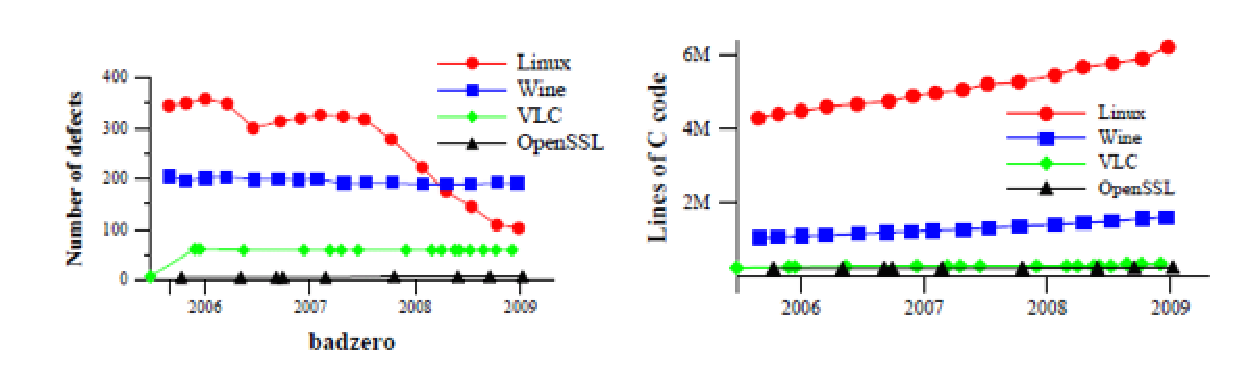
\includegraphics[width=\textwidth]{pic/herograph.eps}
  \caption{各プロジェクトの各世代に対する"badzero"バグの存在数(左図)と各プロジェクトの各世代でのコードサイズ(右図) https://hal.inria.fr/inria-00406306/PDF/RR-6984.pdfから引用}
  \label{herograph}
\end{figure}
\par
図\ref{herograph}から、\acrshort{linux} Kernelはその成長に伴ってbadzeroバグが積極的に改修されているのに対して、その他のプロジェクトでは同種のバグがほぼ放置されたままとなっていることが分かる。
\par
図\ref{heroview}に\acrshort{hero}ワークフローの概要を示す。
\acrshort{hero}は、解析対象となる特定パターンの出現場所が記録された\textcircled{\scriptsize 2}"pattern occurrance reports"と、解析対象となるソフトウェアバージョン間の差分情報\textcircled{\scriptsize 3}"code changes"を入力とする。
ここで、\textcircled{\scriptsize 2}"pattern occurrance reports"は\acrshort{cocci}の出力で、\textcircled{\scriptsize 3}"code changes"は\acrshort{gnu} diffの出力である。
図\ref{heroview}中の"code pattern"は\acrshort{sm}、"pattern matching tool"は\acrshort{cocci}、"diff tool"は\acrshort{gnu} diffを意味する。
"tracking environment"に相当する箇所は、解析対象となるバグパターンを記載した\acrshort{sm}と解析対象の各バージョンのソフトウェアを含めて自前で用意する必要がある。
\textcircled{\scriptsize 4}で\textcircled{\scriptsize 2}"pattern occurrance reports"と\textcircled{\scriptsize 3}"code changes"を受け取った\acrshort{hero}は、入力された特定パターンを入力されたバージョン間にまたがって自動で関係付ける。
ここで、入力されたパターンを\acrshort{hero}が自動的に関係付けられなかったコードについては人間が手動で"SAME"か"UNRELATED"かを判断してラベル付けを行う。
新たに入力されたパターンについては人間が手動で"BUG"か"\acrshort{fp}"かを判断してラベル付けを行う。
つまり最初は全て人間が特定パターンが"BUG"か"\acrshort{fp}"かを\acrshort{hero}に教えるところからスタートする。
このプロセスを回すことによって、過去のバージョンで\acrshort{fp}とラベル付けされ、かつ新しいバージョンでも同じ箇所に同じパターンが残っていると判断されたものについては自動的に\acrshort{fp}のラベルが付与されることになる。
最終的に\acrshort{hero}は特定パターンの時間軸(バージョン毎)における統計情報とグラフを出力する。
\begin{figure}[ht]
  \centering
  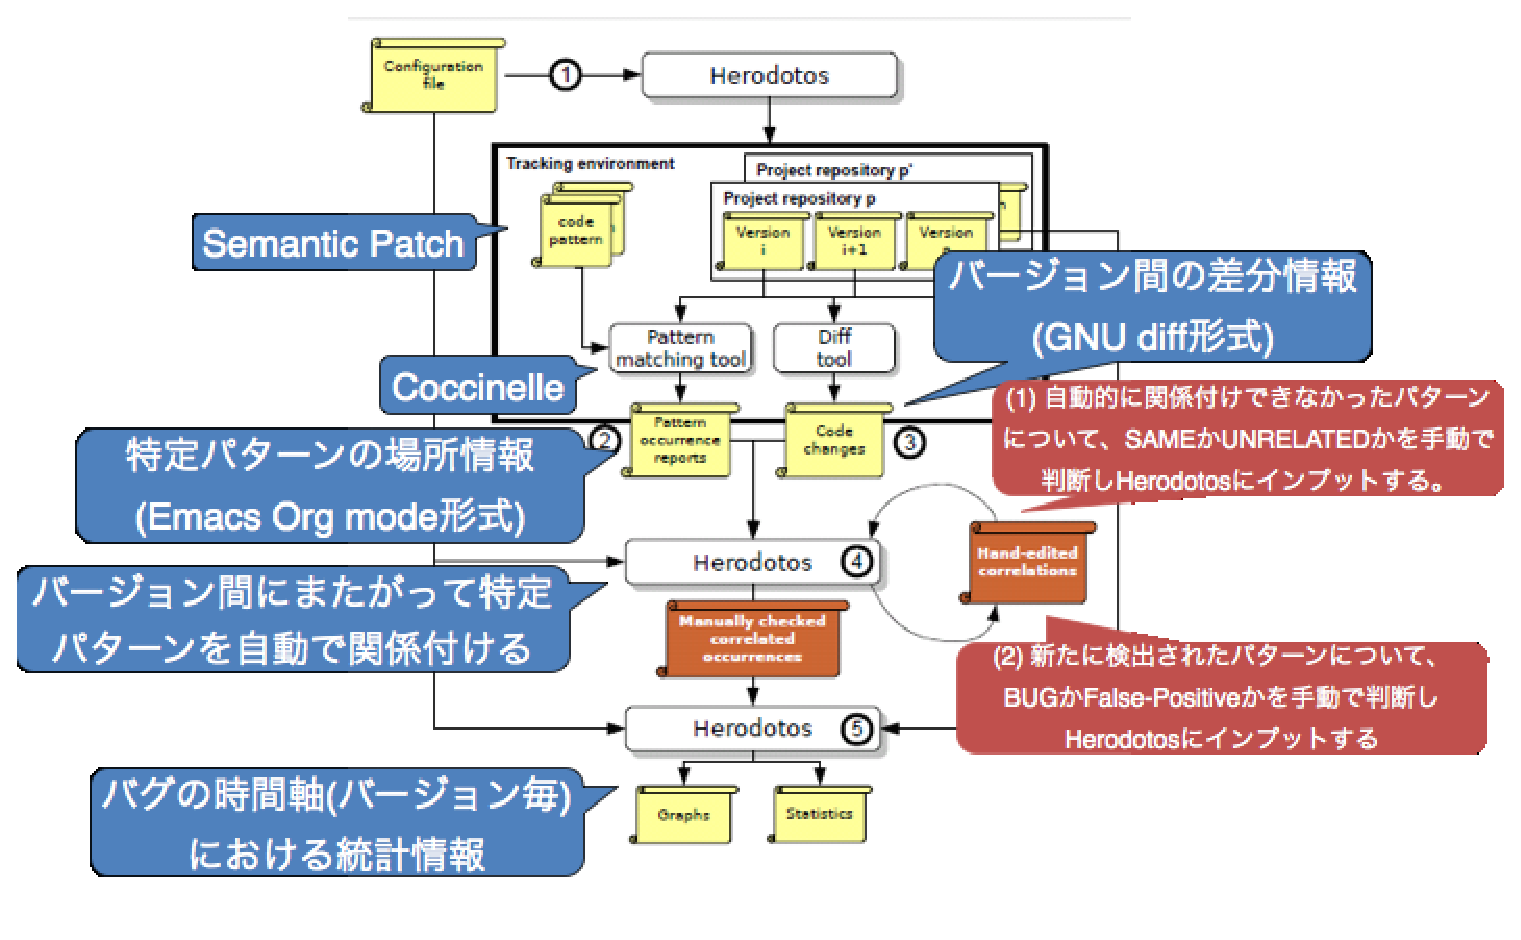
\includegraphics[width=\textwidth]{pic/heroview.eps}
  \caption{\acrshort{hero}のワークフロー}
  \label{heroview}
\end{figure}
\par
なお、\acrshort{cocci}に限らず一般に\acrshort{fp}を抑制する方法としては、使用するkernel configに基づいて無効な \verb|#ifdef| コードブロックを削除する前処理を行うことでビルド対象だけからなるソースコードを抽出し、検査対象となるソースコードそのものを絞るという方法も有りうる。この手法は\ref{mini}節で詳述する。
\subsubsection{Prequel}
\label{presec}
%\acrshort{pre}は\acrshort{cocci}と\acrshort{hero}と同じく\acrshort{inria}が開発中の、セマンティックパターンサーチをコミット履歴(パッチ)に対して行うツールである。
\acrshort{pre}はセマンティックパターンサーチをコミット履歴(パッチ)に対して行うツールで、\acrshort{cocci}と\acrshort{hero}と同じく\acrshort{inria}が開発している。
\acrshort{cocci}がソースコード空間に対してセマンティックパターンサーチを行うのに対して、\acrshort{pre}はサーチ対象を時間軸であるコミット履歴(パッチ)に拡張する。
\acrshort{pre}は開発中のためまだツールの実態は存在しないが、主に次の目的で利用されることが想定されている。
\begin{itemize}
  \item ある修正を行いたい場合に、過去に似たような修正が行われていないかを探すことでその適切な修正方法や副作用を調査する。
  \item 過去に行われた修正で現在のコードの別の箇所にも同じ修正を適用するべきパターンが残存していないかを探し、同じ問題が繰返し発生することを防止する。
  \item コミットログを解析し、各開発者に対するメトリクス(スキルレベルや危険なコードを書く可能性など)を測る。
\end{itemize}
\subsubsection{bugspots}
\acrshort{sil2linuxmp}で取り上げられた手法ではないが、\acrshort{pre}と関連してコミット履歴を元にバグ予測を行う手法に次のようなものが知られている。
\href{http://google-engtools.blogspot.sg/2011/12/bug-prediction-at-google.html}{Googleが2011年に公開したバグ予測アルゴリズム} \cite{google}によると、「バグ修正が最近頻繁にコミットされている箇所ほど残存バグがある可能性が高い」という経験則がある。
Googleでは毎日大量のコードコミットがあり人手によるレビューを全ての変更に対して十分に行うことは現実的に不可能であるため、バグがある可能性が高い"hot spot"に集中してレビューを行う必要がある。
そのようなhot spotを特定するために、trial \& errorの末に導かれた式が(\ref{google})である。
\begin{equation}
  Score = \sum_{i = 0}^{n} \frac{1}{1 + e^{-12t_{i} + 12}}
\label{google}
\end{equation}
\par
ここで、$n$はバグ修正に関連するコミットの数、$t_i$は$i$番目のバグ修正コミットのタイムスタンプでこの値は$0 \sim 1$で正規化されている。
$0$はソースコードベースで最初のコミットがあった時点を表し、$1$は現時点を表す。つまり式(\ref{google})を評価する時点によって$t_i$の値は変動する。
式(\ref{google})は新しいバグ修正ほど大きく重み付けされ、過去のバグ修正ほど小さく評価されるようスケーリングされている。
これをグラフに描くと図\ref{hotspot}のようになる。
\begin{figure}[ht]
  \centering
  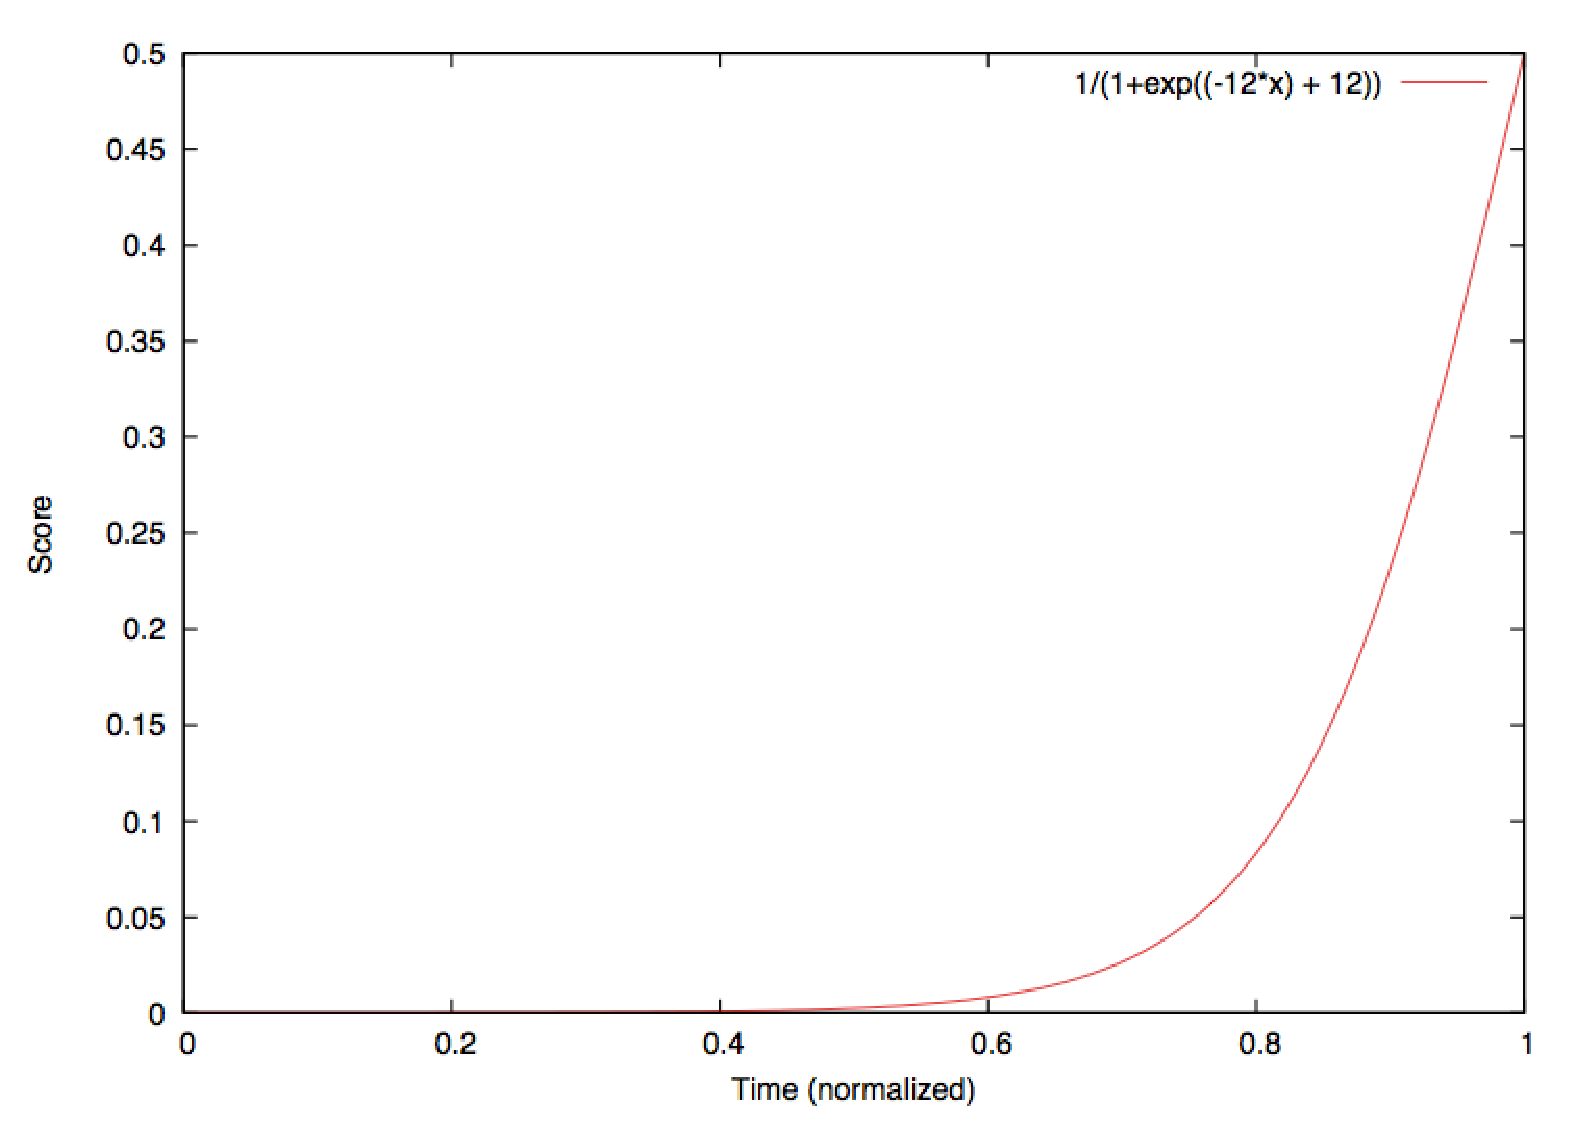
\includegraphics[width=0.8\textwidth]{pic/hotspot.eps}
  \caption{バグが残存する可能性が高いhot spotを評価する式(\ref{google})のグラフ}
  \label{hotspot}
\end{figure}
\par
式(\ref{google})の$Score$が一定の閾値を超える箇所に絞って集中的にコードレビューやコストのかかる検証を行うことで、ソフトウェアの品質を効率良く向上させることができる。
これはバグ修正のコミットタイミング情報のみを利用するごく単純な方法であるが、他のバグ予測アルゴリズムを抑えてバグの出現傾向を良く近似しているという。
\href{https://github.com/igrigorik/bugspots}{\acrshort{bugspot}} \cite{bugspot}はこのhot spot特定技法の\acrshort{rb}によるオープンソース実装である。
\newpage
\subsection{プロジェクト管理}
機能安全対応の開発においては開発対象のソフトウェアそのものに対する正当性検証に加えて、要求と設計のトレーサビリティなどマネジメント観点でのエビデンスを体系的に残し、開発プロセスが健全であることを認証機関に説明することも求められる。
次に\acrshort{sil2linuxmp}で採用が検討されているプロジェクト管理ツールを述べる。
\subsubsection{OGSN}
\label{ogsn}
\gls{gsn}は、達成すべき目的・性質・品質についてそのゴールを実現するための戦略・道筋・方法・思考を可視化するためのアシュアランスケース記法の一つである。
\acrshort{gsn}はEvidence Chainを記述するための国際的な標準表記法であり\acrshort{iso26262}で採用されている。
機能安全対応の際は特にSafety Case Conceptについて、思考の過程を共有し系統立てて議論を進め「なぜその方法で目的が達成できるのか」を認証機関に説明するために\acrshort{gsn}表記が用いられる。\\
 \href{http://blogs.itmedia.co.jp/hiranabe/2013/11/goal-structuring-network.html}{参考ブログエントリ:\acrshort{gsn}(Goal Structuring Notation)解説} \cite{gsne}
\par
\acrshort{gsn}表記は、長方形で示されたゴールが複数のサブゴールにブレークダウンされ、それらが最終的に円で示されたエビデンスまたはソリューションで支えられる構造を取る。
ゴール(長方形)とエビデンス(円)の間には戦略が平行四辺形で記述され、その戦略の根拠や仮定が楕円で、ゴールを目標として成立させている前提条件が角丸長方形で表現される(図\ref{gsn})。
\begin{figure}[ht]
  \centering
  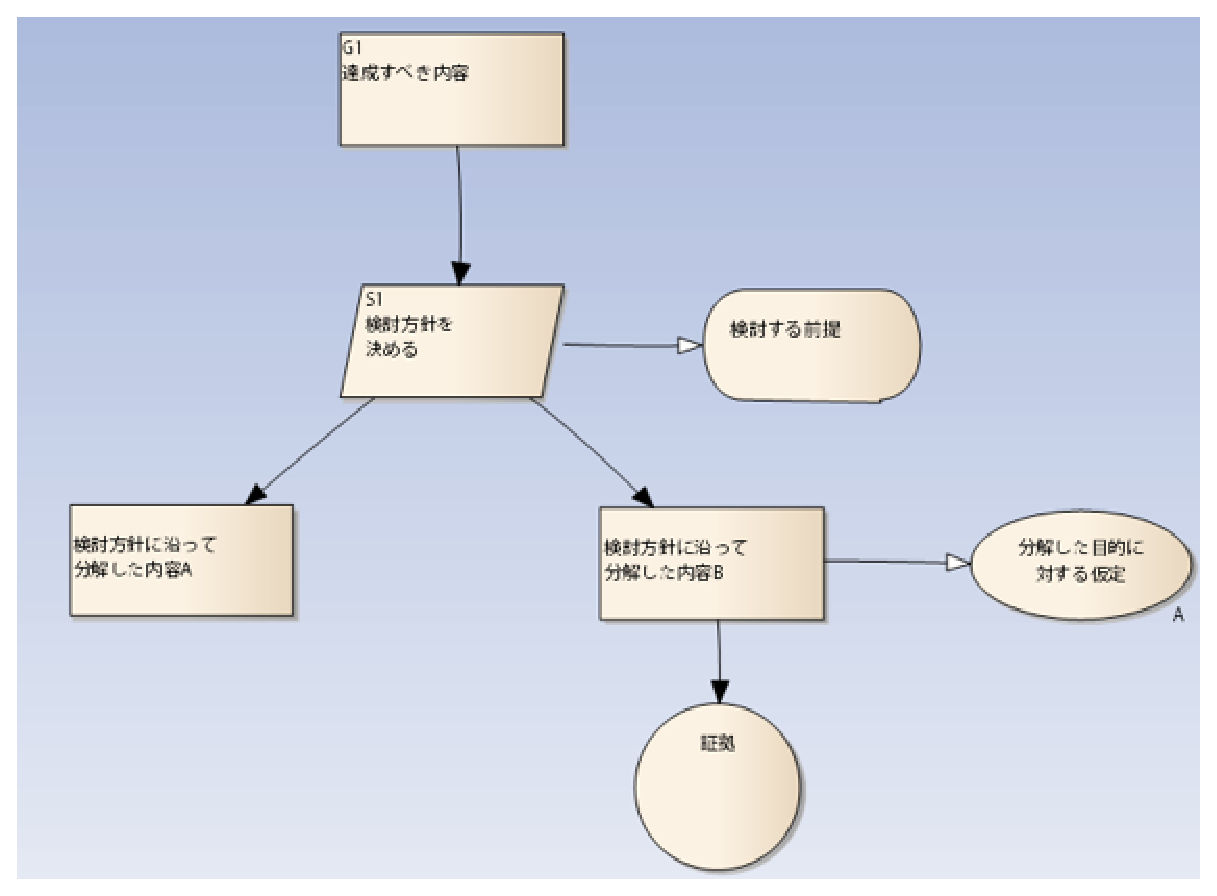
\includegraphics[width=0.9\textwidth]{pic/gsn.eps}
  \caption{\acrshort{gsn}表記の基本的な構造}
  \label{gsn}
\end{figure}
\par
\acrshort{sil2linuxmp}ではSafety Caseを\acrshort{gsn}表記で記述するためのエディタとして既存のツールが利用可能であるかが調査されたが、最終的に\acrshort{sil2linuxmp}プロジェクトで独自に\gls{ogsn}を開発することとなった。\acrshort{iec61508}-3 7.4.4.3 には、off-line 開発ツールの選定条件および選定根拠が明示されることとの記述がある。これに従い\acrshort{sil2linuxmp}では\acrshort{gsn}エディタに求めるマネジメント要件と機能要件として次の項目を挙げた。
\begin{itemize}
  \item マネジメント要件
  \begin{itemize}
    \item プロジェクトの初めから最後まで利用できることが保証されていること
    \item 様々な開発プラットフォーム上で利用可能であること
    \item 将来にわたっても利用できる実行できること
    \item オープンソースライセンスであること
  \end{itemize}
  \item 機能要件
  \begin{itemize}
    \item \acrshort{gsn}コミュニティが定める\href{http://www.goalstructuringnotation.info/documents/GSN\_Standard.pdf}{\acrshort{gsn}標準記法} \cite{gsn} Part1で定義された\acrshort{gsn}基本要素に対応していること
    \item \href{http://www.goalstructuringnotation.info/documents/GSN\_Standard.pdf}{\acrshort{gsn}標準記法} \cite{gsn} Annexes A1とB1の特に"Away Goal"表記に対応していること
  \end{itemize}
\end{itemize}
\par
上記で定めた要件をクライテリアとして、3つの\acrshort{gsn}エディタ\acrshort{dcase}、\acrshort{acedit}、\acrshort{advocate}が調査された。
\acrshort{gsn}エディタには商用で利用できるものが多数存在するが、それらはオープンソースライセンスでないため選定候補にはならない。
調査を行った既存の\acrshort{gsn}ツールと各々の特徴概要は次の通りであった。
\begin{itemize}
  \item \href{http://wiki.portal.chalmers.se/agda/pmwiki.php?n=D-Case-Agda.D-Case-Agda}{\acrshort{dcase}} \cite{dcase}
  \begin{itemize}
    \item \acrshort{eclipse}上で動く\acrshort{java}実装の拡張\acrshort{gsn}エディタ
    \item 厳密な\acrshort{gsn} standardに従っていない独自の表現がある
    \item 保守が止まっていて2010年の\acrshort{eclipse}でないと使えない
  \end{itemize}
  \item \href{https://code.google.com/p/acedit/}{\gls{acedit}} \cite{acedit}
  \begin{itemize}
    \item \acrshort{eclipse}上で動く\acrshort{java}実装の拡張\acrshort{gsn}エディタ
    \item \acrshort{dcase}よりも\acrshort{gsn}標準に従っている。
    \item \acrshort{eclipse}プラグインのインストールに難あり
  \end{itemize}
  \item \href{http://ti.arc.nasa.gov/m/profile/edenney/papers/sassur2012.pdf}{\acrshort{advocate}} \cite{advocate}
  \begin{itemize} 
    \item \acrshort{eclipse}上で動く\acrshort{java}実装の拡張\acrshort{gsn}エディタ
    \item グラフ要素の形が\acrshort{gsn}標準からかけ離れている
    \item \acrshort{eclipse}プラグインのインストールに難あり
    \item ホームページの最終更新が2011年
  \end{itemize}
\end{itemize}
\par
調査の結果、各ツールともメンテナンス状況が十分でないことと\acrshort{eclipse}に付随するバージョン・プラグイン依存関係が複雑であることから、\acrshort{sil2linuxmp}では既存ツールから適切なものを選定する方針を改め、独自にシンプルで必要最小限の\acrshort{gsn}エディタ\gls{ogsn}を開発することとなった。
\acrshort{ogsn}は120行程度の\acrshort{py}スクリプトであり、必要最小限の依存ライブラリ(ConfigParse, PyGraphviz)を持ち、\acrshort{gsn}グラフ表現では\acrshort{gv}を使用して自動的にノード・エッジを配置する仕組みとなっている。
\acrshort{ogsn}は\acrshort{sil2linuxmp}コアメンバーの\acrshort{ot}がプロトタイプを開発中で、今後は次の課題を中心に実装が進められる予定である。
\begin{itemize}
  \item \acrshort{gsn}標準記法の違反・例外チェック(ループ検出等)作りこみ
  \item \acrshort{gsn}標準で定められた記法の順次適用
  \item \acrshort{gsn}グラフ表示形式の洗練、Sub Treeの導入
  \item 複数分割ファイル入力のサポート
\end{itemize}
\subsubsection{rmToo}
\acrshort{sil2linuxmp}プロジェクトにおいて、開発履歴のトレーサビリティは\acrshort{git}で、目標(ゴール)からエビデンス・ソリューションへのトレーサビリティは\acrshort{ogsn}で確保されるが、これのみでは安全要求の開発履歴や要求間および要求と\acrshort{gsn}で表現した目標やソリューションとのトレーサビリティを取ることができない。
そこで\acrshort{sil2linuxmp}では\acrshort{gsn}エディタと同様にシンプルなオープンソースの要求管理ツールとして\href{http://rmtoo.florath.net}{\gls{rmtoo}} \cite{rmtoo}の使用が検討されている。
\par
\acrshort{rmtoo}は\acrshort{py}で実装されたシンプルなコマンドラインツールであり、Plain Textで書かれた要求事項からHTMLまたはPDF形式でのドキュメントや要求項目間の依存関係グラフを出力する。
\acrshort{rmtoo}には\acrshort{gui}や専用のエディタは付随しない。テキストベースの\acrshort{cui}ツールであるという特性は\LaTeX{}と親和性が高く、\acrshort{sil2linuxmp}の\gls{srs}文書は\LaTeX{}に\acrshort{ogsn}で描いた図と\acrshort{rmtoo}が併用されて要求間のトレーサビリティが考慮された構成となっている。
ツールの成熟度は高いが、\acrshort{rmtoo}がただ一人の開発者によって書かれていることと、\acrshort{gh}上の更新が2012年12月で止まっておりメンテナンス状況が不透明であることが懸念点として挙げられている。
\subsection{その他}
本節で詳しく述べることはしないものの、\acrshort{sil2linuxmp}で利用することが検討されているツール、または\acrshort{oss}・\acrshort{linux}開発において標準的に用いられているツールとして次のようなものがある。
\begin{description}
  \item[トレーシング・プロファイリング:]ftrace, kprobes, perf
  \item[カバレッジメトリクス測定:]gcov/lcov
  \item[ベンチマーキング:]lmbench, hackbench, crashme
\end{description}
\par
新たな開発ツールの採用を検討するときは、\ref{ogsn}項の\acrshort{gsn}エディタ選定で行ったようにツールに求める要件とクライテリアを定めて、各ツール候補についてアセスメントを行った上で適切なツールを選ぶ。
または要件を満たす既存ツールがなければ独自に新規開発を行う判断をする。
独自に新規開発を行う場合は、\acrshort{iec61508}が示す3通りの規格準拠方法(\pageref{3route}ページ)のうち$1_S$(初めから最後まで全て厳格に品質管理されたプロセスの下で開発・評価を行う)に従うことになる。
\newpage
\section{SIL2LinuxMPの戦略と規格準拠プロセスの理解}
\label{sil2process}
\ref{tool}節では、\acrshort{sil2linuxmp}プロジェクトでの利用が検討されているツール類のうち代表的なものを述べた。
本節では、機能安全対応開発においてツールセットを選択するための戦略と、既存ツールを組み合わせて新たなエビデンスを得る方法について\acrshort{sil2linuxmp}で検討されているアイディアを記載する。
\subsection{SIL2LinuxMPのツール選定戦略}
\label{toolselection}
\acrshort{sil2linuxmp}の開発基本方針はRoute \textbf{$3_S$}: assessment of non-compliant development(規格非適合の箇所に対して対策を行い適合と証明するに十分な根拠を与える)である。
このことは、従来の開発プロセスにおいて「設計・実装」に相当するフェーズが既存ソフトウェアの「選定」に置き換わるを意味している(図\ref{dlc})。
\begin{figure}[ht]
  \centering
  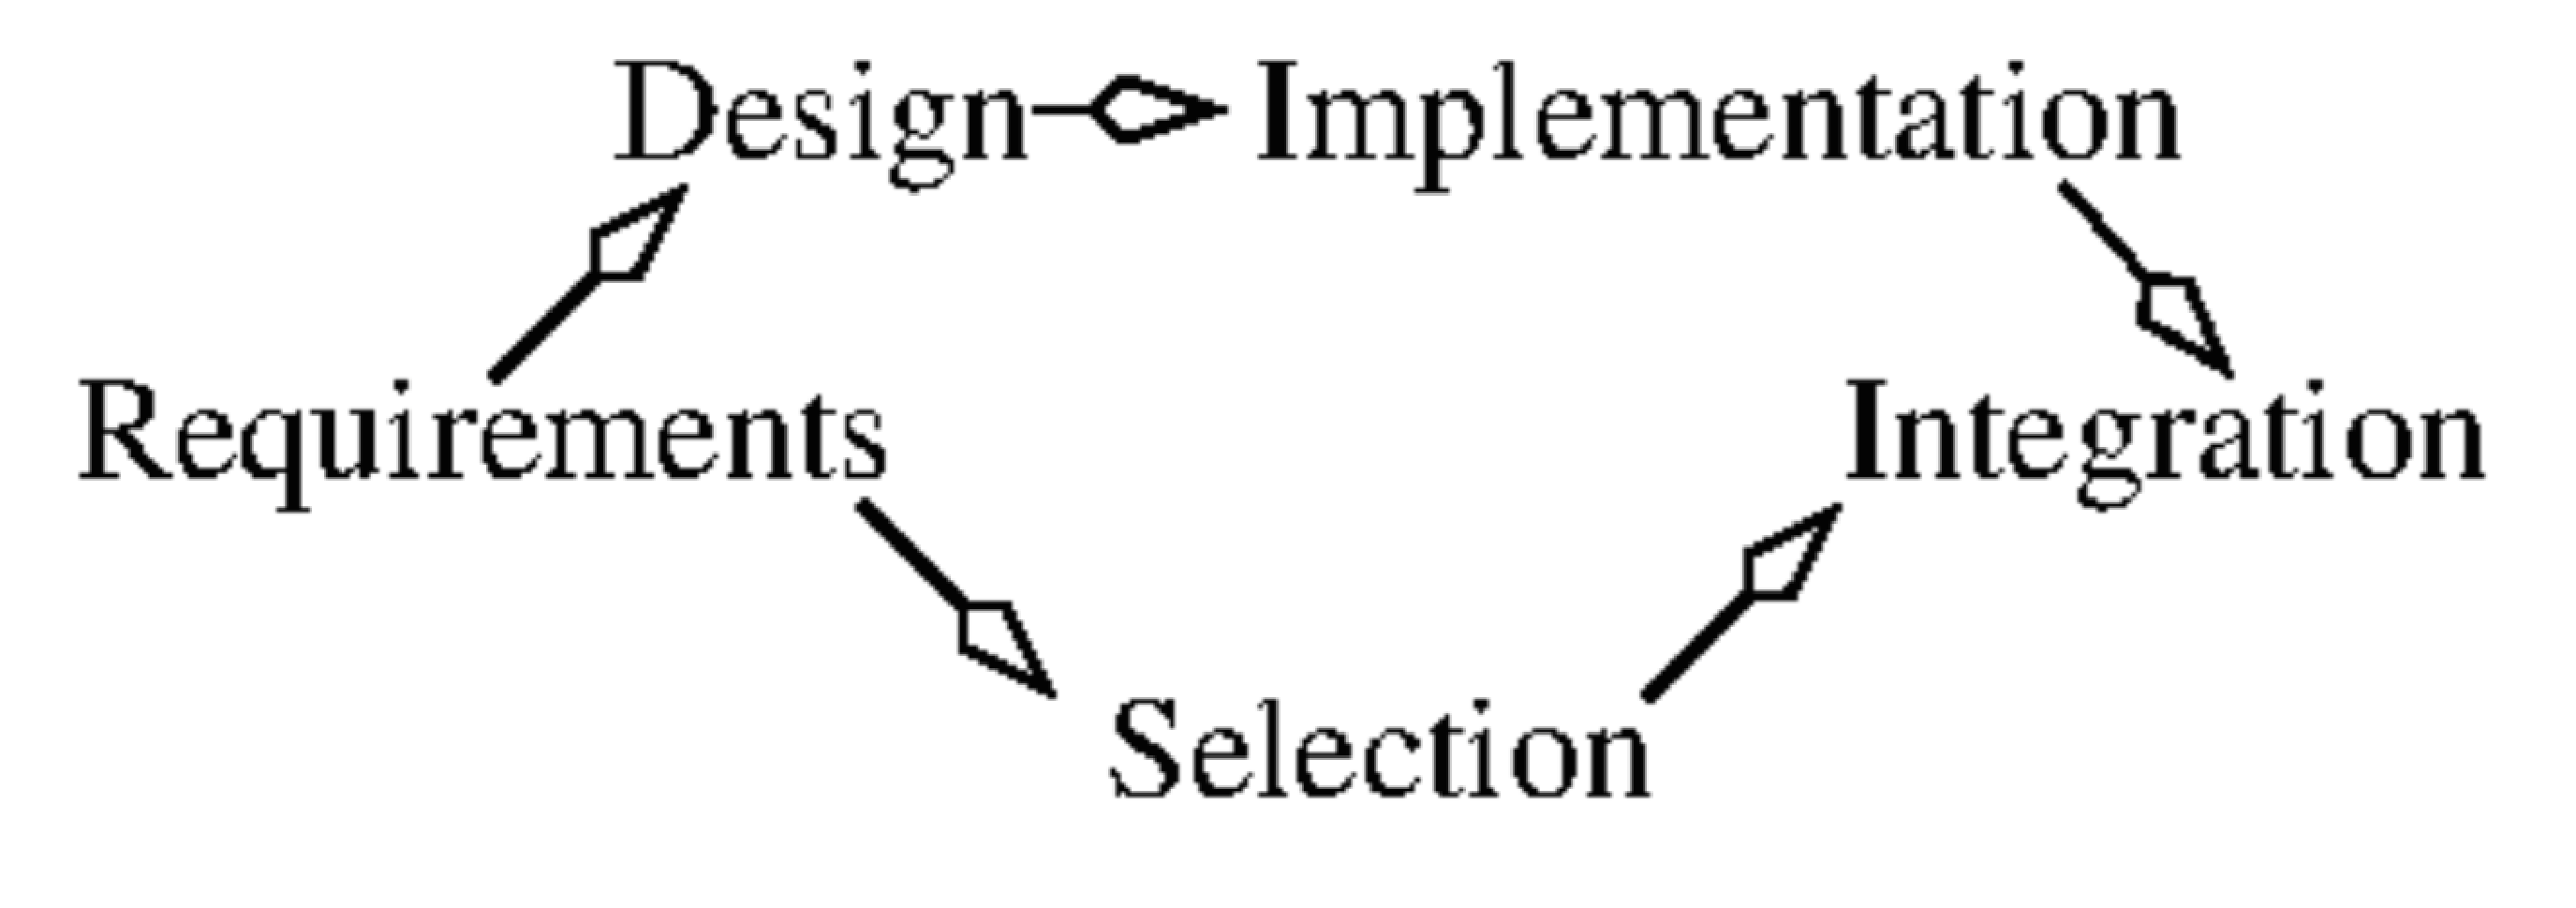
\includegraphics[width=0.7\textwidth]{pic/DLC.eps}
  \caption{既存ソフトウェアの選定プロセスが中心となる開発プロセスへの変化}
  \label{dlc}
\end{figure}
\par
選定フェーズの入り口ではソフトウェアに対する要求として選定クライテリアを定め、出口では定めたクライテリアに対する既存ソフトウェアのアセスメント結果を用意する。
既存ソフトウェアそれ自体が十分な品質・安全性を保証できない場合はそれを補うエビデンスを生成できる手段やツールを新たに導入する。
新たなツールの導入に関して特に考慮すべき事項は以下の通りである。
\begin{itemize}
  \item 非機能要件(実行環境・言語・依存ツール・使用方法)
  \item 機能要件(最低限備えるべき機能・あれば良い機能)
  \item カスタマイズの自由度
  \item コミュニティの成熟度と実績
\end{itemize}
\par
導入するツール自体についてもそれを採用する妥当性を認証機関に証明することが求められる。
ここでツール自体が多機能かつ大規模で複雑であったり、実行環境が特殊であったり、依存物が多かったりすると
精査しなければいけない対象と調査コストが現実的でない規模にまで膨らんでしまう。
そのため機能安全開発で使用するツールとしては、妥当性を証明できるほど十分に小さい構成と簡単な依存関係を持ち、かつ一般に広く認知されていて既に実績がある技術を使用したものが有利である。
\par
また新しいツール導入の際は、既に使用している開発ツールセットとの整合性もツール選定の基準となる。
同じ開発プラットフォーム上で動作するか、依存物の競合を起こさないか、バージョンの組み合わせは問題ないかなどを精査し、全体の開発ツールセットが「一貫した整合性を持つ必要最小限の構成」となるよう考慮する。
必要最小構成のツールセットを実現するためには、例えば使用しない機能を無効にすることでその部分の妥当性検証を省略する戦略が考えられる。
その場合は設定をオープンに操作できるカスタマイズ自由度があるツールほど有利である。
\subsubsection{スケールする検証フレームワークを実現するための戦略}
\label{scale}
\acrshort{sil2linuxmp}に特有の事情として、認証対象がオープンソースソフトウェアであるという点がある。
このことは、認証対象の妥当性を示すためのエビデンスを生成する検証ツールもオープンソースでなければならないことを意味する。
vendor lock-inを回避するため、かつ認証対象ソフトウェアのバージョンアップに追従するため、それらに対する検証は全てオープンな技術に基づいて開発者自身が実施できるものである必要がある。
このような要件に対応するためには何らかの検証自動化の工夫が不可欠である。
加えて、過去に実施したテストケースなどの資産を漸増的に繰返し再適用でき、さらにソースコードのアップデートに基づいて自動的にテストケースが追加生成されることで
その検証フレームワークを回せば回すほど自動的に品質を裏付けるエビデンスが蓄積されていくような仕組みを構築できれば、開発プロセスをスケールすることができる。
\ref{tool}節で述べたツールは各々、このような「スケールする検証フレームワーク」の一要素となる特性を持っている。
\acrshort{cocci}は過去に明らかになったバグを\acrshort{sm}で一般化・蓄積し回帰テストに用いることで同種のバグが新たに発生することを未然に防ぐことができる。
\acrshort{csmith}はランダムテストケースを生成し続けることでテスト母数を増やし品質の裏付けとなるエビデンスを蓄積することができ、
蓄積されたテストケースはソフトウェアのバージョンアップに対する回帰テストとして繰返し適用できる。
そして\acrshort{sil2linuxmp}では新たに\acrshort{fuzzer}の一種である\acrshort{syzkaller}の調査検討が進められているように、
「スケールする検証フレームワーク」を構築するためにはテストケースを自動生成できてそれを蓄積し回帰テストで繰返し適用できるような性質を持つ技術要素が特に有効であると考えられる。
\par
しかし図\ref{QA_Tasks}で述べた通り、品質管理ライフサイクルにおいてはテスト実行やテストケース生成にとどまらず、バグ抽出(\acrshort{fp}フィルタリング)、バグレポート生成、バグ管理、メトリクス測定・テストレポート生成など様々なタスクを実施する必要がある。
「スケールする検証フレームワーク」を構築するためには、これらのタスクを含めた品質保証エコシステム全体を自動化する工夫が必要となる。
特に問題となると考えられるのは「テストケース生成」と対になる「バグ抽出」の自動化である。
\acrshort{cocci}と\acrshort{csmith}の項目で述べた通り、これらは出力に大量の\acrshort{fp}が含まれるという共通の課題を持つ。
\acrshort{inria}が\acrshort{cocci}に対する\acrshort{fp}抑制策として\acrshort{hero}や\acrshort{pre}を提案しているが、これらはまだ人手の介入度合いが多く実績も少ない。
検証ツール全体を見渡しても、\acrshort{fuzzer}に代表されるテストケース生成自動化のためのツール・手法は豊富にあるものの、大量のテスト結果から真のバグをシステマティックに抽出する技法はほぼ存在しないように思われる。
テストケース生成を自動化した結果大量の\acrshort{fp}が出力され、その選別のために人手が必要である限り「スケールする検証フレームワーク」は実現できない。
テストケースを継続的に管理する仕組み構築に対して、テスト結果から真のバグを選別する何らかのバグトリアージの仕組みが不可欠である(図\ref{eco})。
\begin{figure}[ht]
  \centering
  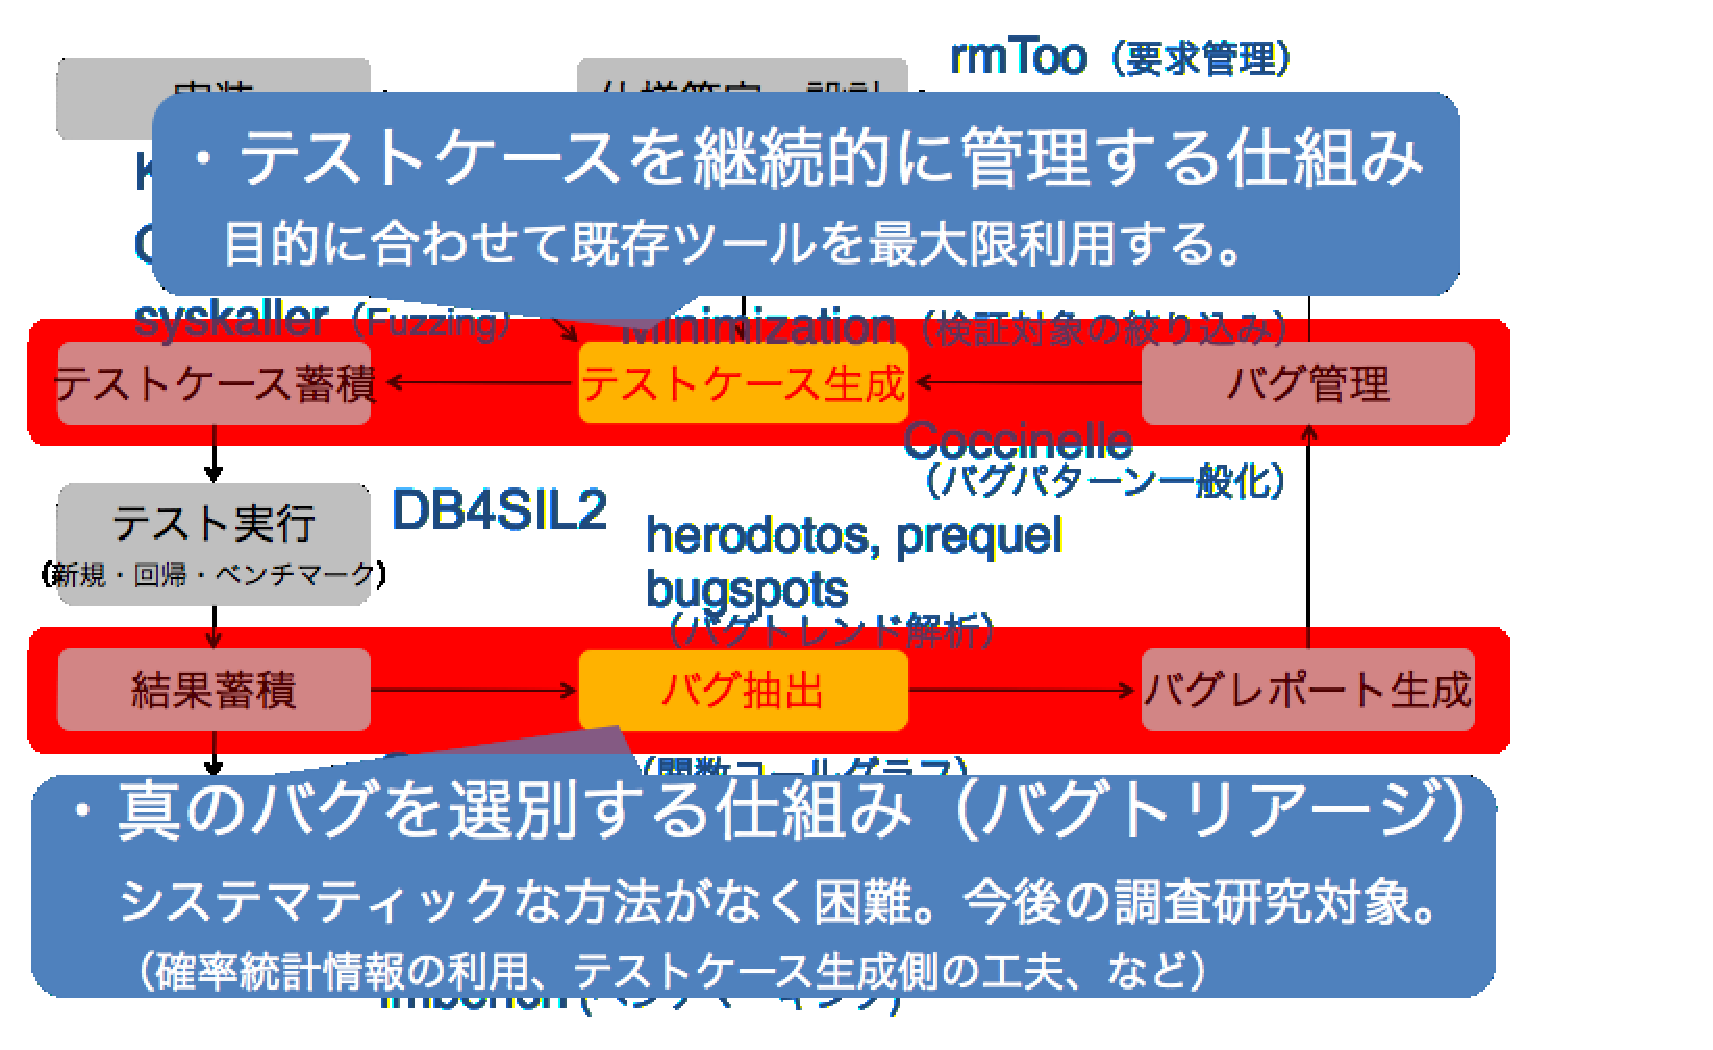
\includegraphics[width=0.95\textwidth]{pic/eco.eps}
  \caption{品質保証エコシステムにおいて対となるテストケース生成部分とバグ抽出部分}
  \label{eco}
\end{figure}
\par
バグトリアージという言葉は一般には「大量の不具合から優先して対処すべき案件を選別する」ことを意味するが、図\ref{eco}では「大量の\acrshort{fp}を含む不具合から真に不具合である案件を選別する」という拡張した意味で用いている。
テスト対象に応じて既存ツールから適切なテストケース生成ツールを選定するように、バグ抽出も対応の仕方はテスト結果の形式次第となる。
ただしここで場当たり的な\acrshort{fp}選別ではなく、\acrshort{bugspot}のように確率統計情報を用いて真のバグが残存する可能性が高い箇所を絞り込むことや、そもそも\acrshort{fp}を出力させない工夫をテストケース生成側で施すことなど、システマティックなバグトリアージ手法を確立する工夫が必要である。
具体的なバグトリアージ手法は今後の調査研究課題である。
\subsection{統合検証フレームワーク:DB4SIL2}
\label{db4sil2sec}
\acrshort{iec61508}-3 Table B.2 - Dynamic analysis and testing(図\ref{100})の7a$\sim$7dでは、各種カバレッジ$100\%$を達成することが\gls{sil2}で\gls{r}または\gls{hr}とされている。
ここで、カバレッジ測定のための技法は対象となるソフトウェアの特性に従って適切に選択されなければならない。
Table B.2の通り$100\%$カバレッジが達成できない場合はカバーできない箇所に対する合理的な説明を与えるか、カバーできない部分を特定し何らかの代替手段で補うことが求められている。
\begin{figure}[ht]
  \centering
  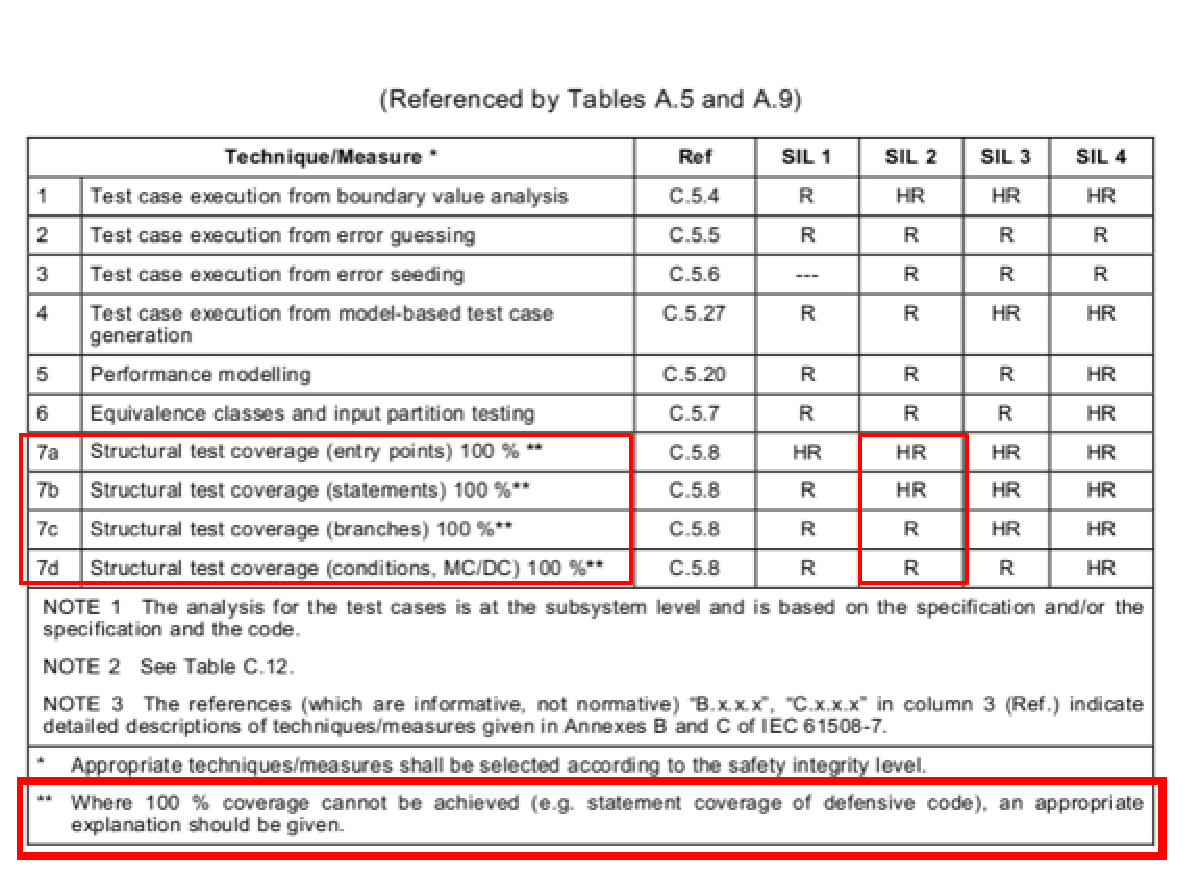
\includegraphics[width=\textwidth]{pic/100.eps}
  \caption{\acrshort{iec61508}-3 Table B.2 - Dynamic analysis and testing}
  \label{100}
\end{figure}
\par
一般にカバレッジを測定するテスト手法には、対象となる\acrshort{oss}ソフトウェアを開発するコミュニティで標準で使われている手法・ツールを用いる。
例えば\acrshort{linux} Kernelであれば\acrshort{ltp}や\acrshort{posix}を利用することをまず検討する。
その上で、既存の手法・ツールではカバーできない領域を特定し、そのようなコード領域へ何らかの対策を行う。
カバーされないコード領域への対策としては例えば次の\ref{enum:prove}, \ref{enum:makeup}ような戦略が考えられる。
\begin{enumerate}
  \item 該当コードが実行され得ないことを示してテスト不要であることを証明する \label{enum:prove}
  \item 該当コードをテストするテストケースを何らかの手段で生成する \label{enum:makeup}
\end{enumerate}
\par
戦略\ref{enum:prove}(テスト不要箇所の特定)の具体例としては、コンパイル対象とならないデッドコードを特定してそもそも検証対象から外す方法があり得る。
このデッドコードを除外する手法については\ref{mini}節で詳述する。
または、\acrshort{cpa}による形式検証手法により到達し得ないコードを特定して検証対象から外す根拠とすることも考えられる。
戦略\ref{enum:makeup}(テストケースの補完)については、例えば\acrshort{klee}による\acrshort{se}ツールで必要なカバレッジを達成するテストケースを(半)自動生成することが考えられる。
このように、コード内部構造の理解に基づいて\acrshort{black}テストのパフォーマンスを向上させる戦略は\textbf{\acrshort{gb}テスト}と呼ばれることがある。
\acrshort{sil2linuxmp}プロジェクトでは、\acrshort{gb}テストをはじめ\acrshort{oss}・\acrshort{linux}の機能安全対応に必要な検証技法を実装するための統合検証フレームワークとして\gls{db4sil2}を開発している。
\acrshort{db4sil2}の開発では、予め定められたクライテリアによって選定された検証ツールセットが統合され、ツール同士が入出力データをやり取りし互いにエビデンスを補完しあう形で図\ref{eco}のような品質保証エコシステムを構築することを目指している。
\begin{figure}[ht]
  \centering
  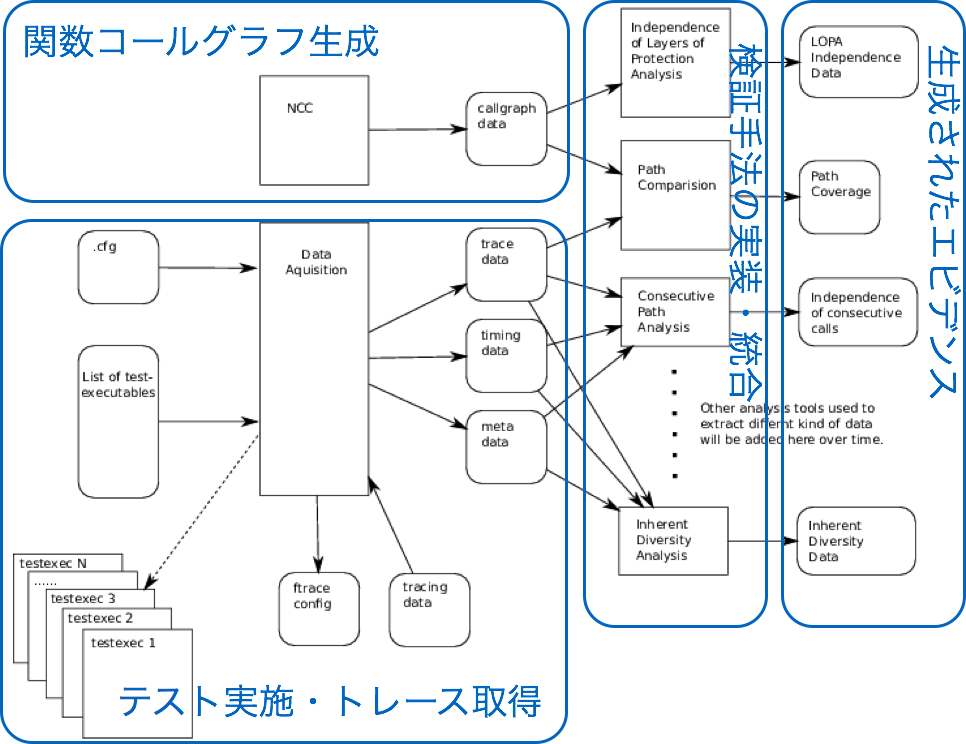
\includegraphics[width=\textwidth]{pic/db4sil2big.eps}
  \caption{\acrshort{db4sil2}の構想:機能安全認証に必要なエビデンスを生成する仕組みを実装・統合する}
  \label{db4sil2big}
\end{figure}
\par
図\ref{db4sil2big}は現時点での\acrshort{db4sil2}の構想である。\acrshort{db4sil2}は関数コールグラフやトレーサなど既存ツール
で得られるデータを入力とし、機能安全認証プロセスで求められる様々なエビデンスを生成する。以降で
は必要なエビデンスを得るために\acrshort{db4sil2}開発で具体的に検討されている検証手法を述べる。
\subsubsection{関数コールグラフとトレーサを用いたカバレッジ解析手法}
\label{callgraph}
\acrshort{gb}テストを行うためには、実施されたテストでカバーされていないコード領域を特定することが前提として必要である。
本章では、関数コールグラフとトレーサを用いてカバレッジ解析を行う手法として\acrshort{db4sil2}開発で検討されている戦略を述べる。
\begin{figure}[ht]
  \centering
  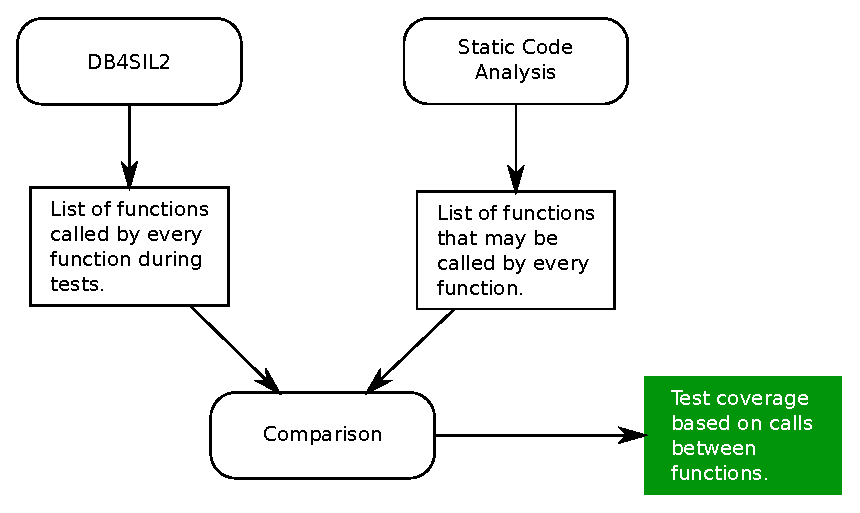
\includegraphics[width=0.85\textwidth]{pic/cov.eps}
  \caption{関数コールグラフとトレーサを用いたパスカバレッジ測定方法}
  \label{cov}
\end{figure}
\par
図\ref{cov}は、事前にソースコードの静的解析によって得られた関数コールグラフと、テストによって得られた動的トレース結果を付き合わせることでパスカバレッジに関するメトリクス解析を行うワークフローである。
ここで、静的関数コールグラフを得るためには\ref{cv}項で記載した\acrshort{cv}を使用する。
\acrshort{cv}のnccを使い関数ポインタを介した呼び出し関係までを静的に解析することで、対象とするソースコードにおいて実行される可能性のある関数呼び出しパスを全てリストすることができる。
動的トレースの取得には\gls{ftrace}を用いる。\acrshort{ftrace}は、kernel空間の動的挙動に対するデバッグや障害・性能解析ツールとして広く使われている\acrshort{linux} Kernelの機能であり、
予め埋め込まれたトレースポイントを契機として関数呼び出し履歴と各々の関数の実行時間を低負荷で記録することができる。
ここで、実行され得る関数呼び出し関係を\acrshort{cv}を使いソースコードを基に全て洗い出した上で、そのソースコードでビルドしたソフトウェアで任意の動的テストを行ったときの関数呼び出し履歴を\acrshort{ftrace}で取得することを考える。
これによって得られた静的関数コールグラフと動的関数コールグラフを比較した結果、静的グラフに存在するが動的グラフには出現しない関数呼び出しパスが特定されれば、そのパスが実施されたテストでカバーされていない部分であると言うことができる。
また、その比較解析結果から関数呼び出しパスについてのカバレッジメトリクスを測定することができる。
\par
例えば、システムコール\verb|SyS_sched_getscheduler()|を契機に呼ばれる可能性のある関数は\acrshort{cv}の関数コールグラフ導出により明らかになる(図\ref{getscheduler})。
ここで、あるテストを行った結果\acrshort{ftrace}によるトレースが図\ref{getscheduler}中のTrace1, Trace2のように得られたとする。
Trace1, Trace2中で現れた関数呼び出しパスをコールグラフ中で探すと、コールグラフで\checkmark{}を付けたエッジが見つかる。
\checkmark{}を付与していないエッジがカバーされていない関数呼び出しパスに相当する。
\begin{figure}[ht]
  \centering
  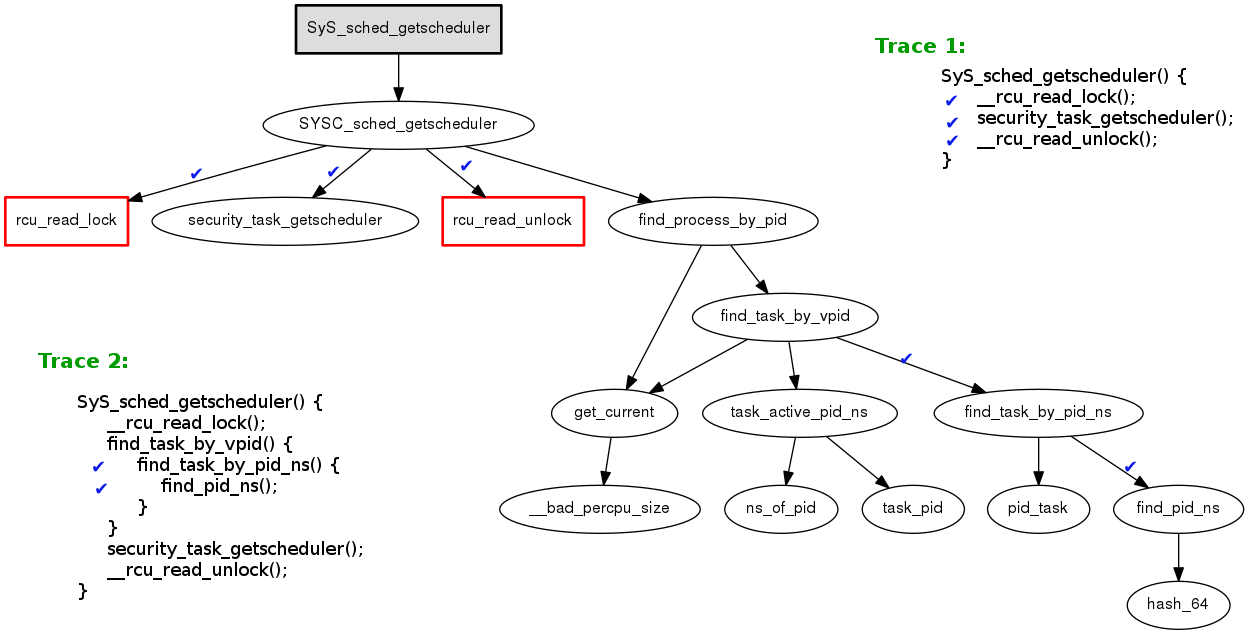
\includegraphics[width=\textwidth]{pic/getscheduler.eps}
  \caption{関数コールグラフとトレーサを用いたパスカバレッジ測定例}
  \label{getscheduler}
\end{figure}
\par
本項で述べた解析手法によって得られ得た静的・動的関数コールグラフは、ソースコードに変更が入った際にその全体への影響を調べるインパクトアナリシスにとっても有用なデータとなる。
変更が加えられた関数を直接・間接的に呼んでいる関数、または変更箇所から呼ばれている関数が既に明らかであれば、変更の全体への影響を調べるためには関数コールグラフ上変更箇所と関係を持つコード領域のみに注目してレビューや回帰テストを実施すればよい。
データを介したやり取りや、イベント・割り込みが関わる直接的な関数呼び出しでない非同期挙動の分析はこの限りではないが、インパクトアナリシスの範囲を考えるための一つの指標として用いることができる。
\par
以上のような関数コールグラフとトレーサを用いたカバレッジ測定手法およびインパクト解析手法は、\acrshort{ftrace}の性質上適用できる範囲がカーネル空間のみに制約される。
しかし\acrshort{sil2linuxmp}プラットフォームとして\acrshort{sil2}対応の目標となっている領域には\acrshort{linux} Kernelに加えて\acrshort{bb}と\acrshort{glibc}からなる最小構成のユーザ空間も含まれる。
そのため、同様の手法をユーザ空間でも適用するべきであると\acrshort{sil2linuxmp}コミュニティでは認識されており、
ユーザ空間における具体的ツールと実現手段は今後の調査検討課題となっている。
\subsubsection{関数コールグラフのLOPAへの応用}
\label{sil0}
機能安全対応のシステム開発では、必ずしも常にシステム全体に同一の安全水準が求められるわけではない。
システム要求や開発リソース・コストなどのマネジメント戦略次第で、特定の部分のみ\acrshort{sil2}水準の安全性を確保しその他の部分は\acrshort{sil0}(\gls{qm}:安全性の要求なし)領域とするアーキテクチャ設計も可能である。
ただし、このように複数の安全水準を持つサブシステムを混在させる場合は各領域の影響が互いに干渉することのないように対策を施さなければならない。
特に\acrshort{sil0}(\acrshort{qm})非安全領域で欠陥や障害があった場合にその影響が\acrshort{sil2}安全領域に伝搬することは許容されない。
\acrshort{sil2}安全領域と\acrshort{sil0}(\acrshort{qm})非安全領域との隔離を実現する手段のひとつとして、\acrshort{sil2linuxmp}では図\ref{isol}のように\acrshort{linux}コンテナ技術を利用した構成が検討されている。
\begin{figure}[ht]
  \centering
  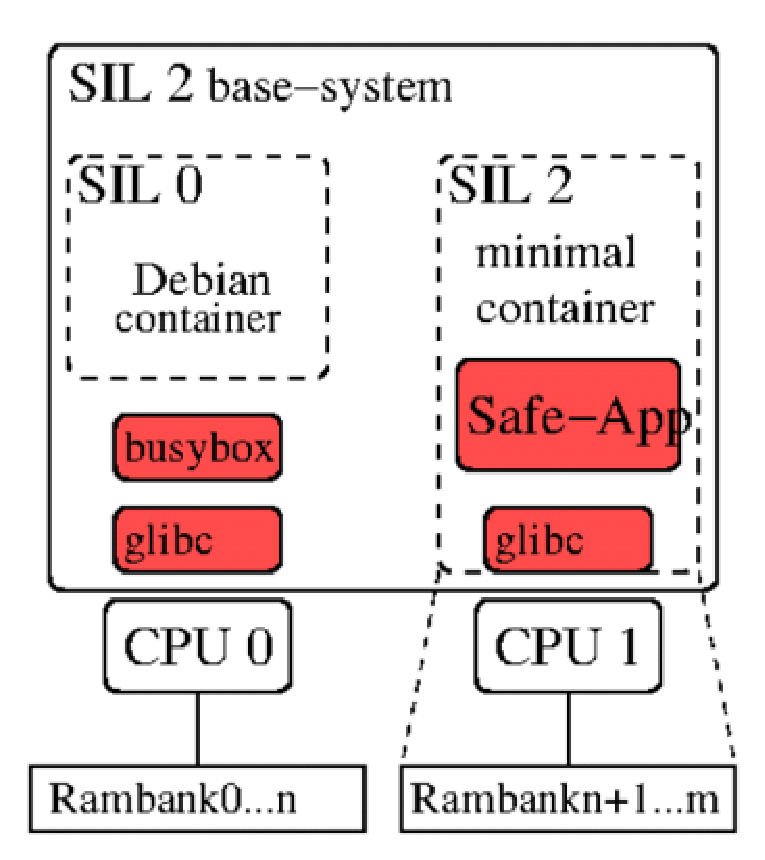
\includegraphics[width=0.45\textwidth]{pic/isol.eps}
  \caption{\acrshort{sil2}安全領域と\acrshort{sil0}(\acrshort{qm})非安全領域をコンテナで隔離するシステム構成}
  \label{isol}
\end{figure}
\par
\acrshort{gnu}/\acrshort{linux}システムにおける一般的なコンテナ技術はユーザ空間から見たリソースを各々のコンテナ内で隔離するものであるが、厳密にkernel内部のリソースまで隔離して運用することはできない。
そのため、本来安全に隔離保護されているべき領域に対するリスク評価を行う\gls{lopa}の実施が求められる。
\acrshort{sil2linuxmp}では\acrshort{db4sil2}開発の一環として、関数コールグラフを利用した\acrshort{lopa}実施方法が次のように検討されている。
%\paragraph{ \acrshort{seccomp}と\acrshort{cgroups}のリソース独立性を解析する例}
%\par
\subsubsection{\acrshort{seccomp}と\acrshort{cgroups}のリソース独立性を解析する例}
\gls{cgroups}はプロセスのリソース(CPU、メモリ、ディスクI/O等)の利用を制限または隔離する\acrshort{linux} Kernelの仮想化機能である。
\gls{seccomp}はユーザ空間に対してシステムコールの利用を制限したサンドボックス環境を提供する\acrshort{linux} Kernelのセキュリティ機能である。
\acrshort{cgroups}と\acrshort{seccomp}はともに、ユーザ空間のアプリケーションを隔離することで他のアプリケーションやシステムにその挙動の影響を伝搬させないことを意図して使われることが一般的である。
互いにその挙動が独立であることが想定されているならば、各々の機能から使われる関数も呼び出し関係は分離されているはずであると予想される。
ここで、\acrshort{cgroups}と\acrshort{seccomp}の両方の機能を無効にしたときに使われるコード領域に含まれる関数の集合を$BASE$、
\acrshort{seccomp}だけを有効にしたときの領域に含まれる関数の集合を$SEC$、
\acrshort{cgroups}だけを有効にしたときの領域に含まれる関数の集合を$CGR$として各々の関係を考える(図\ref{bs})。
\begin{figure}[ht]
  \centering
  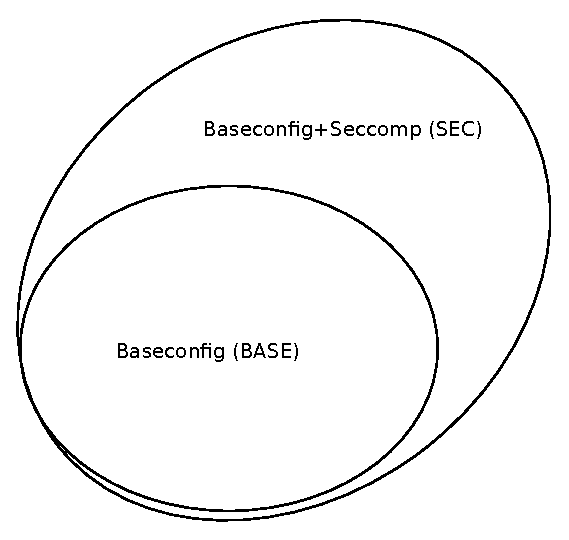
\includegraphics[width=0.6\textwidth]{pic/bs.eps}
%  \caption{\acrshort{seccomp}機能を有効にしたときのコード領域\verb|SEC|と\verb|SEC|に無関係なベース領域\verb|BASE|}
  \caption{\acrshort{seccomp}機能を有効にしたときに使われる関数の集合$SEC$と、無効にしたときの関数の集合$BASE$}
  \label{bs}
\end{figure}
\par
\acrshort{seccomp}機能と\acrshort{cgroups}機能が独立であるならば$SEC$と$CGR$の共通部分は$BASE$の部分集合であるはずであるが、$SEC$と$CGR$の共通部分に属しかつ$BASE$に属さない関数
%\newline
($ \in (SEC \cap CGR) \smallsetminus BASE$)が存在する(図\ref{intersec})。
このような共通部分に属する関数は、各々\acrshort{seccomp}機能と\acrshort{cgroups}機能に関する関数コールグラフを導出することで調べることが可能である。
\acrshort{seccomp}と\acrshort{cgroups}から共通して使われる関数が特定されれば、それらの共通関数に範囲を限定してレビューや検証のコストを集中させることで各々の機能の独立性を効率的に調査することができる。
つまり本項で述べた戦略は機能の挙動が完全に隔離されていることの証明を目指すのではなく、各々から共通して参照される範囲を特定した上で
その限定された部分が共通して参照されても問題ないことを示すかまたは必要に応じて何らかの対策を施すという、
\acrshort{iec61508}-3 7.4.2.12 Route $3_S$: assessment of non-compliant development の原則に基づくものである。
\begin{figure}[ht]
  \centering
  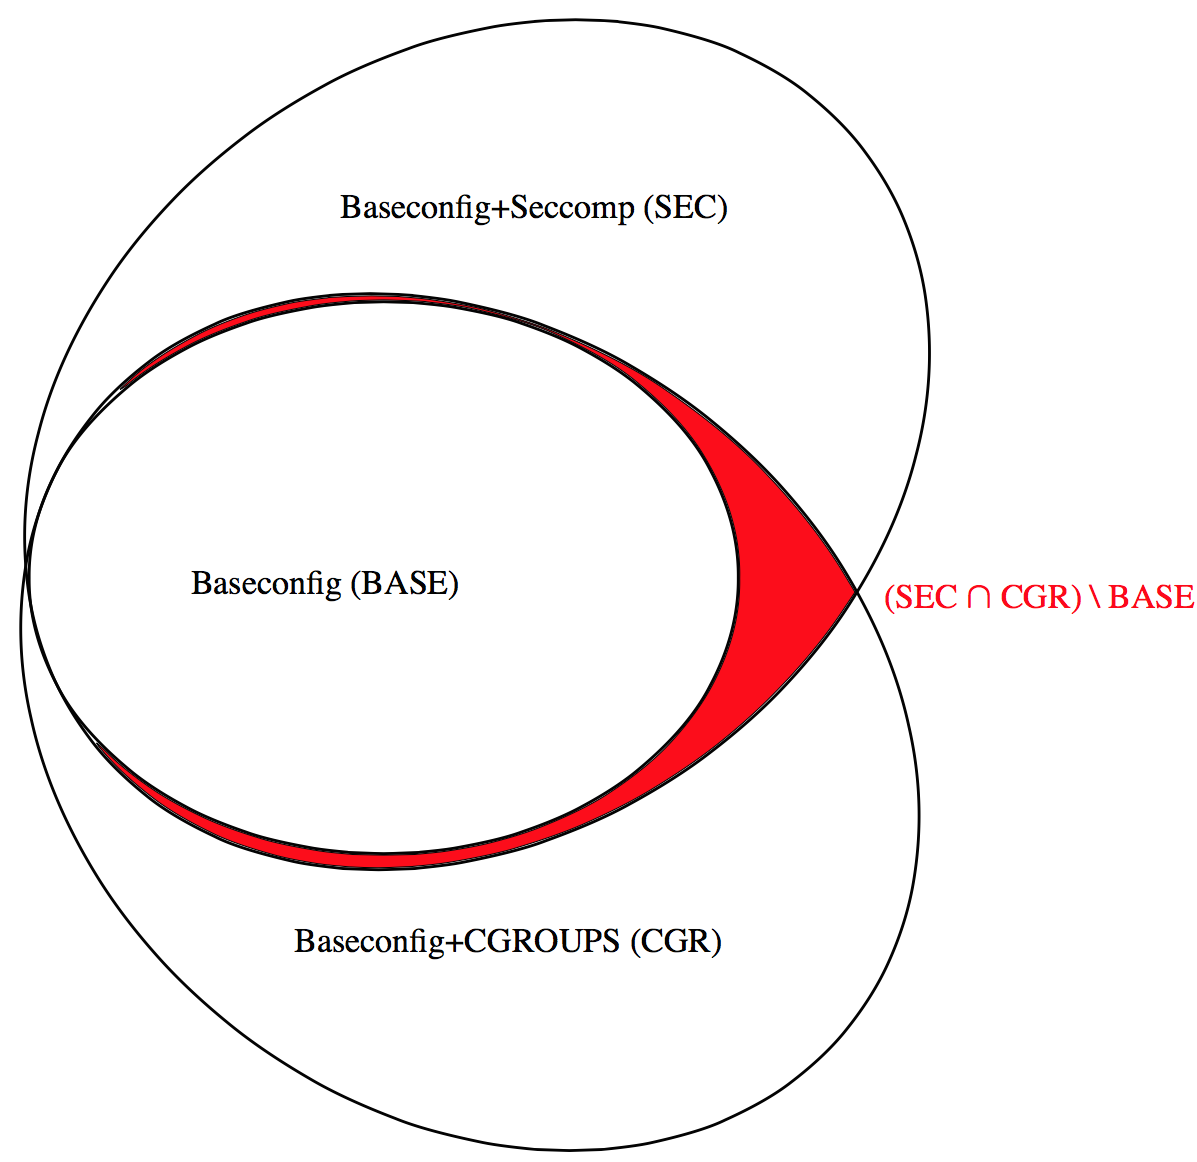
\includegraphics[width=0.8\textwidth]{pic/intersec.eps}\
  \caption{$(SEC \cap CGR) \smallsetminus BASE \neq \varnothing$}
  \label{intersec}
\end{figure}
\subsubsection{\acrshort{seccomp}と\acrshort{cgroups}の\gls{ccf}分析例}
ソフトウェアの開発履歴情報を共通原因故障(\gls{ccf})分析に応用することが\acrshort{sil2linuxmp}プロジェクトで検討されている。
ソースコードの記述スタイルは各プロジェクト毎に方針が存在し統一されていることが多いものの、コードには開発者毎に思考の癖や好みのパターンが表れる。
そのような開発者依存のコーディングパターンがあるロジック実装で使われたりある別のパターンと併用されたりした場合に
何らかの問題を引き起こす原因となることがあり得る。
オープンソースソフトウェアの開発には\acrshort{git}に代表されるバージョン管理システムが使われることが一般的であり、
そこにはソースコード変更の単位でその開発者名が記録されている。
ここで、例えば\acrshort{seccomp}プロジェクトの\acrshort{git}コミット履歴から\acrshort{seccomp}プロジェクトに参加している開発者を調べれば、
\acrshort{cgroups}プロジェクト側で発生したバグの原因となるコードを書いた開発者が\acrshort{seccomp}のコードにもコミットした履歴があるかどうかが分かる。
この情報を手掛かりにして、\acrshort{cgroups}プロジェクトのバグと同じ原因で発生する可能性のあるバグが\acrshort{seccomp}プロジェクトにも残存する可能性をさらに分析することができる。
\par
ちなみに\acrshort{seccomp}と\acrshort{cgroups}の両方のプロジェクトにコミット履歴を残している開発者と各コミット数は表\ref{deveopers}の通りである。
\begin{table}[hb]
  \caption{\acrshort{seccomp}と\acrshort{cgroups}に共通する開発者と各コミット数}
  \label{deveopers}
  \centering
  \begin{tabular}{ll|ll}
    \multicolumn{2}{c|}{\acrshort{seccomp}} & \multicolumn{2}{c}{\acrshort{cgroups}} \\
    \hline 
    54 & Linus Torvalds & 2 & Linus Torvalds \\
    52 & Daniel Borkmann & 203 & Daniel Borkmann \\
    48 & David Howells & 3 & David Howells \\
    2 & Fabian Frederick & 1 & Fabian Frederick
  \end{tabular}
\end{table}
